%%%%%%%%%%%%%%%%%%%%%%%%%%%%%%%%%%%%%%%%%%%%%%%%%%%%%%%%%%%%%%%%%%%%%
%%                                                                 %%
%% Please do not use \input{...} to include other tex files.       %%
%% Submit your LaTeX manuscript as one .tex document.              %%
%%                                                                 %%
%% All additional figures and files should be attached             %%
%% separately and not embedded in the \TeX\ document itself.       %%
%%                                                                 %%
%%%%%%%%%%%%%%%%%%%%%%%%%%%%%%%%%%%%%%%%%%%%%%%%%%%%%%%%%%%%%%%%%%%%%

%%\documentclass[referee,sn-basic]{sn-jnl}% referee option is meant for double line spacing

%%=======================================================%%
%% to print line numbers in the margin use lineno option %%
%%=======================================================%%

%%\documentclass[lineno,sn-basic]{sn-jnl}% Basic Springer Nature Reference Style/Chemistry Reference Style

%%======================================================%%
%% to compile with pdflatex/xelatex use pdflatex option %%
%%======================================================%%

%%\documentclass[pdflatex,sn-basic]{sn-jnl}% Basic Springer Nature Reference Style/Chemistry Reference Style

%%\documentclass[sn-basic]{sn-jnl}% Basic Springer Nature Reference Style/Chemistry Reference Style
\documentclass[sn-mathphys]{sn-jnl}% Math and Physical Sciences Reference Style
%%\documentclass[sn-aps]{sn-jnl}% American Physical Society (APS) Reference Style
%%\documentclass[sn-vancouver]{sn-jnl}% Vancouver Reference Style
%%\documentclass[sn-apa]{sn-jnl}% APA Reference Style
%%\documentclass[sn-chicago]{sn-jnl}% Chicago-based Humanities Reference Style
%%\documentclass[sn-standardnature]{sn-jnl}% Standard Nature Portfolio Reference Style
%%\documentclass[default]{sn-jnl}% Default
%%\documentclass[default,iicol]{sn-jnl}% Default with double column layout

%%%% Standard Packages
%%<additional latex packages if required can be included here>

\usepackage{color,soul}
\jyear{2021}%

%% as per the requirement new theorem styles can be included as shown below
\theoremstyle{thmstyleone}%
\newtheorem{theorem}{Theorem}%  meant for continuous numbers
%%\newtheorem{theorem}{Theorem}[section]% meant for sectionwise numbers
%% optional argument [theorem] produces theorem numbering sequence instead of independent numbers for Proposition
\newtheorem{proposition}[theorem]{Proposition}%
%%\newtheorem{proposition}{Proposition}% to get separate numbers for theorem and proposition etc.

\theoremstyle{thmstyletwo}%
\newtheorem{example}{Example}%
\newtheorem{remark}{Remark}%

\theoremstyle{thmstylethree}%
\newtheorem{definition}{Definition}%

\raggedbottom
%%\unnumbered% uncomment this for unnumbered level heads

\begin{document}

\title[Intensification of FeB association in Si-SCs by acoustic wave]{Intensification of iron-boron complex association in silicon solar cells under acoustic wave action}

%%=============================================================%%
%% Prefix	-> \pfx{Dr}
%% GivenName	-> \fnm{Joergen W.}
%% Particle	-> \spfx{van der} -> surname prefix
%% FamilyName	-> \sur{Ploeg}
%% Suffix	-> \sfx{IV}
%% NatureName	-> \tanm{Poet Laureate} -> Title after name
%% Degrees	-> \dgr{MSc, PhD}
%% \author*[1,2]{\pfx{Dr} \fnm{Joergen W.} \spfx{van der} \sur{Ploeg} \sfx{IV} \tanm{Poet Laureate}
%%                 \dgr{MSc, PhD}}\email{iauthor@gmail.com}
%%=============================================================%%

\author*[1]{\fnm{Oleg} \sur{Olikh}}\email{olegolikh@knu.ua}
%\equalcont{These authors contributed equally to this work.}

\author[2]{\fnm{Vitaliy} \sur{Kostylyov}}\email{vkost@isp.kiev.ua}
%\equalcont{These authors contributed equally to this work.}

\author[2]{\fnm{Victor} \sur{Vlasiuk}}\email{viktorvlasiuk@gmail.com}
%\equalcont{These authors contributed equally to this work.}

\author[2]{\fnm{Roman} \sur{Korkishko}}\email{romkin.ua@gmail.com}
%\equalcont{These authors contributed equally to this work.}

\author[1]{\fnm{Roman} \sur{Chupryna}}\email{r\_chupryna@voliacable.com}
%\equalcont{These authors contributed equally to this work.}


\affil[1]{\orgdiv{Physics faculty}, \orgname{Taras Shevchenko National University of Kyiv}, \orgaddress{\street{64/13, Volodymyrska Street}, \city{Kyiv}, \postcode{01601}, \country{Ukraine}}}

\affil[2]{\orgname{V. Lashkaryov Institute of Semiconductor Physic of NAS of Ukraine}, \orgaddress{\street{41, pr. Nauki}, \city{Kyiv}, \postcode{03028}, \country{Ukraine}}}

%\abstract{The experimental investigation of ultrasound (US) influence on the recovery of light-induced degradation in Si solar cells was performed.
%It was established that degradation is induced by iron-boron pair transformation and the ability of extraction of pair parameters from
%short circuit current kinetics was discussed.
%It was revealed that the application of US loading lead to the acceleration of the FeB pair association.
%This effect was investigated for different US frequencies (0.3--30~MHz) and intensities (up to 1.3~W/cm$^2$) as well as iron concentrations
%((0.2--3)$\times$10$^{13}$~cm$^{-3}$) in the solar cell over temperature range 300--340~K.
%It has been found that US longitudinal waves are more efficient than transverse waves.
%The experimentally observed phenomena are related to the decrease in iron migration energy (up to 10 meV) in the US stress fields.}

\abstract{\hl{In this paper, we study the  influence of ultrasound (US) on the recovery of light-induced degradation in Cz-Si solar cells.
The complete recovery in the dark at near room temperature and the determined value
of activation energy (0.656 eV) evidenced the iron--boron pair transformation-related degradation.}
The ability of extraction of FeB pair's parameters from short circuit current kinetics was discussed.
It was revealed that the US loading leads to the acceleration of the FeB pair association.
This effect was investigated for different US frequencies (0.3--30~MHz) and intensities (up to 1.3~W/cm$^2$) as well as iron concentrations
((0.2--3)$\times$10$^{13}$~cm$^{-3}$) in the solar cell over temperature range 300--340~K.
It has been found that US longitudinal waves are more efficient than transverse waves.
The experimentally observed phenomena are related to the decrease in iron migration energy (up to 10 meV) in the US stress fields.}

%%================================%%
%% Sample for structured abstract %%
%%================================%%

% \abstract{\textbf{Purpose:} The abstract serves both as a general introduction to the topic and as a brief, non-technical summary of the main results and their implications. The abstract must not include subheadings (unless expressly permitted in the journal's Instructions to Authors), equations or citations. As a guide the abstract should not exceed 200 words. Most journals do not set a hard limit however authors are advised to check the author instructions for the journal they are submitting to.
%
% \textbf{Methods:} The abstract serves both as a general introduction to the topic and as a brief, non-technical summary of the main results and their implications. The abstract must not include subheadings (unless expressly permitted in the journal's Instructions to Authors), equations or citations. As a guide the abstract should not exceed 200 words. Most journals do not set a hard limit however authors are advised to check the author instructions for the journal they are submitting to.
%
% \textbf{Results:} The abstract serves both as a general introduction to the topic and as a brief, non-technical summary of the main results and their implications. The abstract must not include subheadings (unless expressly permitted in the journal's Instructions to Authors), equations or citations. As a guide the abstract should not exceed 200 words. Most journals do not set a hard limit however authors are advised to check the author instructions for the journal they are submitting to.
%
% \textbf{Conclusion:} The abstract serves both as a general introduction to the topic and as a brief, non-technical summary of the main results and their implications. The abstract must not include subheadings (unless expressly permitted in the journal's Instructions to Authors), equations or citations. As a guide the abstract should not exceed 200 words. Most journals do not set a hard limit however authors are advised to check the author instructions for the journal they are submitting to.}

\keywords{Ultrasound, Silicon solar cell, Iron-boron pair, Acousto-defect interaction}

%%\pacs[JEL Classification]{D8, H51}

%%\pacs[MSC Classification]{35A01, 65L10, 65L12, 65L20, 65L70}

\maketitle

\section{Introduction}\label{sec1}

It is well known that ultrasound (US) can act efficiently on defect subsystems of semiconductor crystals and devices due to dissipation of US vibration energy, which is particularly intense in the regions with periodicity disorder \cite{ostapenko2002,Savkina2013,Olikh2018JAP}.
At US of \hl{subthreshold} intensity, acoustically induced (AI) reconstruction of defects causes the \hl{reversible} changes in charge concentration and mobility in crystals \cite{Davletova2008,Olikh2020JEM},
barrier height in Schottky structures \cite{Olikh:Ultras,OlikhJAP}
as well as tunnel and recombination currents in p-n structures \cite{Teterkin2009,Olikh2018JAP}.
Also, it seems promising to apply the US as an additional factor of influence during conventional technological processes.
In this case, semiconductor structures are usually found in  nonequilibrium conditions, and the defect--impurity subsystem is capable of modifying easier under the action of elastic oscillations.
For instance, the application of ultrasound loading (USL) \hl{during}  ion implantation facilitates
the formation of ultra-shallow junctions \cite{USImplant:JVacSci}
and intensives the silicon surface layer amorphization \cite{RomanyukSST};
USL applied during the production of porous silicon  results in structural ordering \cite{Kalem2000}
and when applied during ZnO deposition provides higher homogeneity of the films \cite{US:ZnOfilm}.

\hl{ The silicon solar cells (SCs) constitute about 90\% of the global photovoltaic production capacity.
Iron is one of the most relevant, omnipresent, and efficiency--limiting metallic impurities
in p--type Si SCs} \cite{Istratov1999,IronSC}.
\hl{ Therefore, the methods of defect engineering aimed at iron have practical importance.}
In silicon photovoltaics, one of the main methods of impurity deactivation and removing it from the operation zone is gettering Fe atoms at certain centers (extended defects, oxygen precipitates, or interfaces) \cite{LaineIEEEPV2016}.
A similar gettering can be realized during standard operations as phosphorus diffusion \cite{FeB:Vahanissi}
or production of antireflection coating  \cite{Teimuraz2014JAP}.
It is clear that the process efficiency depends on the mobility of iron atoms.

\hl{ On the one hand, shallow acceptors (B, Al, Ga, In) are effective trapping sites for iron around room temperature
and in darkness in p-Si due to electrostatic attraction between the negatively charged
acceptors and the positively charged iron ions.
All Fe-acceptor pairs are similar:
complexes have two structural configurations
with trigonal and orthorhombic symmetry and can be broken by
intense illumination and/or annealing above 200$^\circ$C} \cite{Istratov1999,FeBKinAPL2013}.
\hl{ On the other hand, the back surface field (BSF) cell and passivated emitter and rear cell (PERC)
are the most popular designs that have been used in the mass-production of Si SCs,
and both BSF and PERC are mainly  based on boron-doped silicon wafers }\cite{SCRev2020,GreenRew2019}.
\hl{ Therefore the iron--boron pair is one of the most relevant complexes to the defect engineering in real SCs.}
This work aims to investigate experimentally how acoustic waves (AWs) influence the ability of iron to diffuse in silicon solar cells.
The time of iron--boron pair association after  light-induced dissociation was used as an indicator of iron ion mobility.
The possibility of the ultrasound to  change the state of FeB was shown previously  \cite{Ostapenko1994APL,Ostapenko1995}.
\hl{
In particular, the
FeB pair was revealed} \cite{Ostapenko1995}
\hl{ to be dissociated in Cz-Si by the action of ultrasound with acoustic strain $\xi_\mathrm{US}=10^{-5}$--$10^{-4}$.
Furthermore, Ostapenko and Bell} \cite{Ostapenko1995} \hl{regarded the resonance condition of pair dissociation and used 25--70~kHz.
Besides, it was asserted} \cite{Ostapenko1994APL} \hl{that in the case of
predominant dissociated pairs, the ultrasound may promote the pairing reaction in contradistinction to the case of a
high fraction of paired iron.
But  empirical evidence  for this prediction  is absent.
In this work,
i)~the wave frequency $f_\mathrm{US}=$0.3--30~MHz and subthreshold strain $\xi_\mathrm{US}<2\times10^{-6}$ were used, which were deficient overcome the Coulombic attraction between Fe$_i$ and B$_s^-$;
ii)~the predominant  dissociation of FeB was realized by intense illumination.
Thus the association of FeB pair (the migration  of Fe$_i^+$) was firstly investigated in conditions of USL.}


\section{Experimental and Calculation Details}
\label{sec:1}

Experimental studies were performed on the samples of silicon SC ($1.52\times1.535$~cm$^2$) made based on single-crystal  $p$--type silicon [100] wafers with the resistivity of about 10~$\Omega\cdot$cm
(boron doping level  $N_A=1.4\times10^{15}$~cm$^{-3}$).
The thickness of the wafers was 380~$\mu$m.
\hl{ Diffusion from the gas phase (POCl$_3$) at 940$^\circ$C was performed on wafers resulting in an $n^+$--emitter layer on
the front side (sheet resistance of about $20-30$~$\Omega/\Box$, thickness of $0.7$~$\mu$m).
In addition, to reduce recombination losses and increase the conductivity of the contact layer,
a $p^+$ layer ($10-20$~$\Omega/\Box$, $0.6$~$\mu$m) was formed by boron diffusion from
the gas phase (BCl$_3$) at 985$^\circ$C on the rear surface.}
Layers of SiO$_2$ and Si$_3$N$_4$ were formed on the front surface of the SC to passivate the surface and reduce the optical reflectance.
\hl{ The solid and grid aluminum contacts were formed by magnetron sputtering on the rear and front surfaces, respectively.}
The \hl{schematic structure} of SC is presented in Fig.~\ref{figChem}.
\begin{figure}
\centering
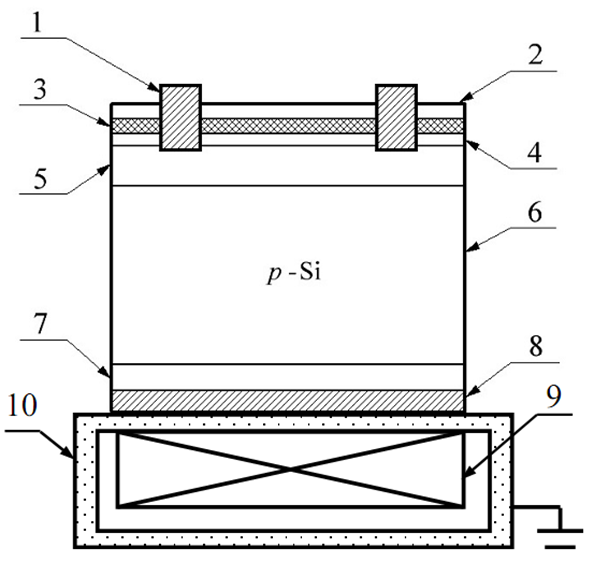
\includegraphics[width=0.5\textwidth]{Fig1}
\caption{\hl{Schematic structure} of the sample and USL.
1 --- frontal \hl{grid} electrode (Al);
2 --- Si$_3$N$_4$ (40 nm);
3 --- SiO$_2$ (30 nm);
4 --- induced $n^{++}$--layer;
5 --- diffusion $n^+$--layer;
6 --- quasineutral base region of $p$--type (350 $\mu$m);
7 --- diffusion $p^+$--layer;
8 --- rear metallization (Al);
9 --- piezoelectric transducer;
10 --- metal foil (Cu)}
\label{figChem}       % Give a unique label
\end{figure}

In the case of USL, the transverse or longitudinal AWs
\hl{were applied to the samples in [100] direction by using LiNbO$_3$ or ceramic piezoelectric transducer}.
The transducer was attached to the whole area of Al back contact.
\hl{It is widely known that the efficiency of ultrasound influence
on  defects in semiconductors depends on acoustic wave frequency $f_\mathrm{US}$.
Moreover, the type of frequency dependence is determined by the mechanism of acousto-defect
interaction} \cite{Brailsford,Pavlovich,PeleshchakUJF2016}.
\hl{ The set of frequencies (2.4, 4.1, 5.4, 9.0, 14, 18, and 31~MHz, longitudinal waves)
was used  to establish features of
ultrasound influence on iron migration.
Besides,  the effect of the increase in the carrier capture coefficient for defects in silicon SC
is shown} \cite{Olikh2018SM} \hl{ to be intensified in the case of the transverse acoustic waves using.
Accordingly, the transverse waves ($f_\mathrm{US}=0.3$~MHz) were used as well.
The ultrasound intensities $W_\mathrm{US}$  did not overcome 1.3~W/cm$^2$.
To} avoid the effect of the piezoelectric field on the measurements procedure \hl{as well as} sample parameters,
the transducer was shielded by Cu foil --- see Fig.~\ref{figChem}.

It is known that Fe in silicon can be in two states:
in the form of FeB pair or in the interstitial state Fe$_i$.
At near room temperature and boron concentration $>10^{14}$~cm$^{-3}$,
almost all Fe bound in FeB pairs is in equilibrium \cite{FeB:kinetic,FeBAssJAP2014,FeBAssSST2011,FeBJAP2005}.
However, numerous researches show that dissociation of pairs can be performed either by heating to the temperature above 200$^\circ$C
or by intense illumination at room temperature \cite{FeBAssJAP2014,FeBJAP2005}.
In our work, we used the latter approach,
and \hl{the high-intensive illumination source} was a halogen lamp
with a radiation intensity of about 250~mW/cm$^2$.
To dissociate Feb pairs, the front side of the sample was illuminated, and the illumination time was  30 s.

\hl{The different light-induced degradation (LID) phenomena exist that affect the efficiency
of Cz-silicon solar cells due to a decrease in the lifetime of generated excess charge carriers.
The main reasons for this transformation are boron--oxygen complex formation (BO-LID)} \cite{LIDRev}
\hl{ and
iron--boron pair dissociation.
Besides, the light- and elevated-temperature-induced degradation (LeTID) is observed.
In recent studies, the occurrence of the LeTID defect is related
to the presence of hydrogen and metal impurities }\cite{LeTID_H,LeTID_Me,LeTID_Me2}.
\hl{ The complete  recovery in the dark at near room temperature and the determined value
of activation energy (0.656 eV, see below) evidenced the iron--boron pair-related LID in our case.}

%It is known that FeB pair dissociations in the SC base are accompanied by the change
%in lifetime of minority carriers $\tau$.
%As an indicator of this quantity we considered short circuit current $I_\mathrm{SC}$,
%which was measured under SC illumination by a low energy monochromatic light source.
%This was a light emitting diode (LED) with radiation power $P_{ph}\sim350$~$\mu$W
%(measured by PowerMeter Rk-5720) and light wavelength $\lambda=940$~nm.
%As the calculations showed, under these conditions the level of nonequilibrium carrier
%excitations was $\Delta n<10^{12}$cm$^{-3}$.

It is known that Feb pair dissociations in the SC base are accompanied by the change
in the lifetime of minority carriers $\tau$.
As an indicator of $\tau$, we considered short circuit current $I_\mathrm{SC}$,
which was measured under SC illumination by a \hl{low-intensive} monochromatic light.
\hl{The low-intensive source} was a light-emitting diode (LED) with radiation
power $P_{ph}\sim350$~$\mu$W (measured by PowerMeter Rk-5720) and
wavelength $\lambda=940$~nm.

%The kinetics of short circuit current was measured after intensive illumination of the sample
%(see Fig.~\ref{figIsc}).
%All the measurements were carried out by varying the temperature from 300 to 340~K with a thermoelectric cooler,
%and by stabilizing it with a computer--controlled PID loop to better than 0.05~K.
%The SC temperature was controlled by STS--21 sensor, which was placed on the front sample surface.

The kinetics of short circuit current was measured after high-intensive illumination
(see Fig.~\ref{figIsc}).
The measurements were carried out over a temperature range
of 300--340~K.
The temperature was varied by a thermoelectric cooler and stabilized by a
computer-controlled PID loop to better than 0.05~K.
The temperature was controlled by STS--21 sensor, which was placed on the front surface of SC.

\begin{figure}
\centering
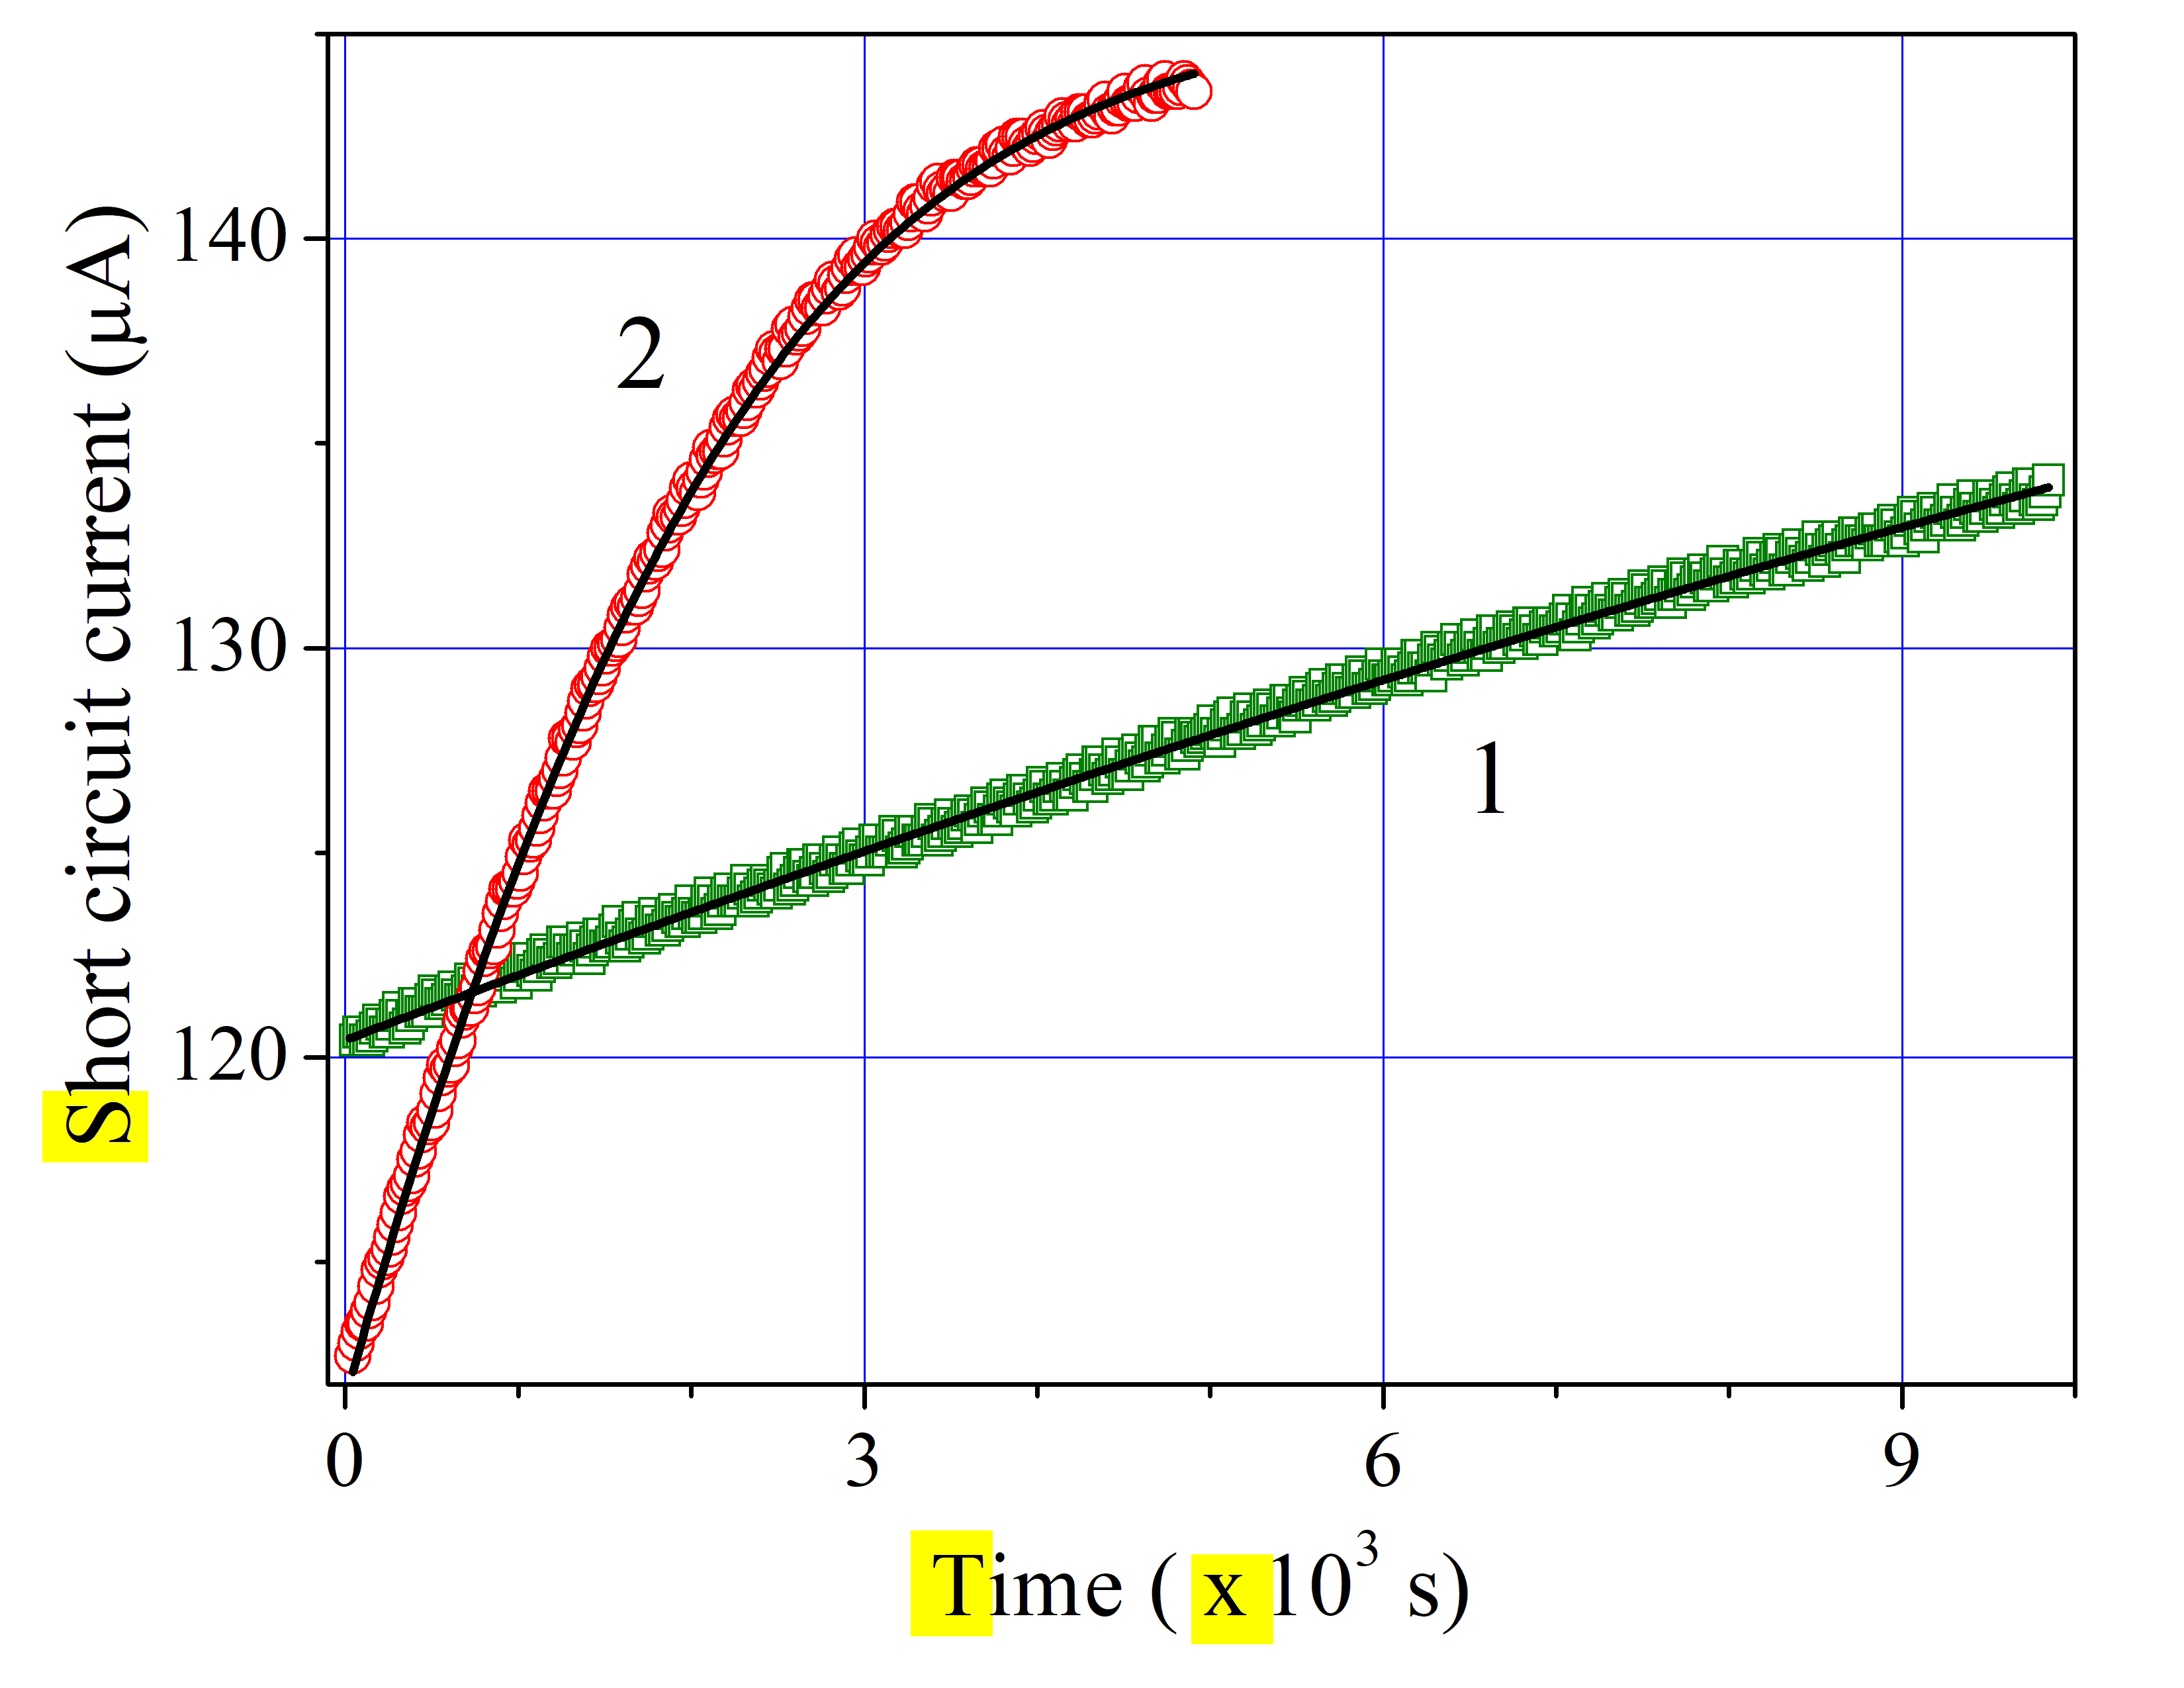
\includegraphics[width=0.5\textwidth]{Fig2}
\caption{
\hl{Measured under low-intensive (LED) illumination short circuit current
 plotted as a function of the time after high-intensive (halogen lamp) illumination.
The marks are the experimental results, the lines are the fitted curves using} Eqs.~(\ref{eqIsc})-(\ref{eqNFeBt}).
\hl{The zero of time corresponds to the moment of intensive illumination termination.}
$T$, K: 300 (1, \hl{ green squares}), 330 (2, \hl{red circles})}
\label{figIsc}       % Give a unique label
\end{figure}

\hl{The FeB pair association in the dark was accompanied by the $\tau$ increase and
was monitored by measuring the $I_\mathrm{SC}$ under LED illumination.
The LED illumination induced excess carrier density $\Delta n<10^{12}$~cm$^{-3}$,
had duty cycle 0.5\% while $I_\mathrm{SC}(t)$ measuring,
and did not cause FeB dissociation.
Moreover, the fitting of the measured dependencies $I_\mathrm{SC}(t)$ after high-intensive illumination
allows determining  the pair concentration and the characteristic time of the FeB complex formation.
In fact, in conditions of homogeneous carrier generation in the base  by the LED illumination,}
the short circuit current can be described as follows \cite{Bube,Razeghi}:
\begin{equation}
\label{eqIsc}
I_\mathrm{SC}(t)=\frac{P_{ph}(1-R_{ph})\,q\beta\lambda}{hc}\frac{\alpha_{ph}L_n(t)}{1+\alpha_{ph}L_n(t)}\,,
\end{equation}
where
\hl{$P_{ph}$ is the LED light power,
$\lambda$ is the light wavelength (940~nm),
$q$ is elementary charge,
$h$ is the Planck constant,
$c$ is the speed of light,}
$\alpha_{ph}=\alpha_{ph}(T,\lambda)$ is the coefficient of light absorption,
which was calculated according to \cite{Si:Absorb,GreenOptic},
\hl{$T$ is the cell temperature,}
$R_{ph}(\lambda)$ is the coefficient of reflection,
\hl{which was calculated for used samples according to} \cite{KostRefl2000,KostRefl2000A}, $R_{ph}$(940~nm)$=0.14$;
$\beta$ is the coefficient of quantum  yield, $\beta=1$;
$L_n$  is the diffusion length of minority carriers.
%$R_{ph}$ is the coefficient of reflection;
%as shown by the calculations with using recurrent correlations for coefficients of amplitude reflections \cite{KostRefl2000,KostRefl2000A},
%in our case from the silicon SC with two layered antireflection coating $R_{ph}$(940~nm)$=0.14$;
%$\beta$ is the coefficient of quantum  yield, $\beta=1$;
%$L_n$  is the diffusion length of minority carriers.
%As the measurements of $L_n$ by spectral dependence of internal quantum yield show,
%the quantity was from 35 to 150~$\mu$m (for different samples),
%which justifies the usage of expression~(\ref{eqIsc}).
In its turn
\begin{equation}
\label{eqLn}
L_n(t)=\sqrt{\frac{\mu_nkT\tau(t)}{q}}\,,
\end{equation}
where
$\mu_n$ is the electron mobility, was calculated by Klaassen theory \cite{KLAASSEN953},
\hl{$k$ is the Boltzmann constant}.


In the assumption that it is the iron-related defects that play an essential role in the recombination,
the following expression can be used to estimate $\tau$ according to Mattisen rule:
\begin{equation}
\label{eqTau}
\tau(t)^{-1}=\tau_{rad}^{-1}+\tau_{Aug}^{-1}+(\tau_{SRH}^{\mathrm{Fe_i}}(t))^{-1}
+(\tau_{SRH}^\mathrm{FeB}(t))^{-1}+\tau_{other}^{-1}\,,
\end{equation}
where
%$\tau_{rad}$ is the lifetime associated with band-to-band radiation recombination
%\begin{equation}
%\label{eqTauRad}
%\tau_{rad}^{-1}=B(N_A+n_0+\Delta n)\,,
%\end{equation}
%$\tau_{Aug}$ is the life time associated with Auger processes:
%\begin{equation}
%\label{eqTauAug}
%\tau_{Aug}^{-1}=C_p\,N_A^2\,,
%\end{equation}
%the values of recombination coefficients $B$ and $C_p$ were calculated by data from \cite{Si_BtB,Si_Auger};
%$n_0=n_i^2/N_A$,
%$n_i$ is the intrinsic carrier concentration, whose dependence on temperature was taken from \cite{Si_ni_Couderc};
%$\tau_{SRH}^{\mathrm{Fe_i}}$  and $\tau_{SRH}^\mathrm{FeB}$ are related to the recombinations at interstitial iron atoms Fe$_i$ and at FeB pairs, accordingly;
%$\tau_{other}$ describes the rest of recombination pathways including surface recombination.
$\tau_{rad}$ and $\tau_{Aug}$ are associated with
band-to-band radiation recombination and Auger processes, respectively;
$\tau_{SRH}^{\mathrm{Fe_i}}$  and $\tau_{SRH}^\mathrm{FeB}$ are related to the
recombinations at interstitial iron atoms Fe$_i$ and at FeB pairs, accordingly;
$\tau_{other}$ describes further
recombination channels including surface recombination.
In turn,
\begin{equation}
\label{eqTauRad}
\tau_{rad}^{-1}=B(N_A+n_0+\Delta n)\,,
\end{equation}
\begin{equation}
\label{eqTauAug}
\tau_{Aug}^{-1}=C_p\,N_A^2\,,
\end{equation}
where the values of recombination coefficients $B$ and $C_p$ were calculated by data from \cite{Si_BtB,Si_Auger};
$n_0=n_i^2/N_A$ and intrinsic carrier concentration $n_i$ was taken from \cite{Si_ni_Couderc}.

In order to calculate $\tau_{SRH}^{\mathrm{Fe_i}}$  and $\tau_{SRH}^\mathrm{FeB}$,
Shockley--Read--Hall model was used:
\begin{equation}
\label{eqTauSRH}
\tau_{SRH}^{\mathrm{Fe_i,FeB}}(t)=\frac{\tau_{p0}(t)(n_0+n_1+\Delta n)+\tau_{n0}(t)(N_A+p_1+\Delta n)}
                             {N_A+n_0+\Delta n}\,,
\end{equation}
where
$\tau_{p0,n0}(t)=(N_{trap}(t) \sigma_{p,n}\upsilon_{th}^{p,n})^{-1}$,
$N_{trap}(t)$ is the \hl{trap} concentration
($N_\mathrm{Fe_i}$ and $N_\mathrm{FeB}$ for Fe$_i$ and FeB, respectively),
$\sigma_n$, $\sigma_p$  are the cross sections of the recombination centers for electrons and holes, respectively,
$\upsilon_{th}^{n}$, $\upsilon_{th}^{p}$ are the average thermal velocities of electrons and holes calculated according to \cite{Nc:Green},
$n_1=N_C \exp(-(E_C-E_t)/kT)$,
$p_1=N_V \exp(-(E_t-E_V)/kT)$;
$N_C$ and $N_V$ are the densities of
states in the conduction band and valence band, respectively \cite{Si_ni_Couderc};
$E_C$ and $E_V$ are the energy of the conduction band and
valence band edge, respectively;
$E_t$ is the energy level of the relevant recombination level.
The parameters of recombination centers related to Fe$_i$ and FeB were taken from \cite{ROUGIEUX2018}.

The time dependence of interstitial iron atom concentration
after pair dissociations is described by the known expression from \cite{MurphyJAP2011}:
\begin{equation}
\label{eqNFet}
N_\mathrm{Fe_i}(t)=(N_\mathrm{Fe_i,0}-N_\mathrm{Fe_i,eq})\cdot
\exp(-t/\tau_{ass})+N_\mathrm{Fe_i,eq}\,,
\end{equation}
where
$\tau_{ass}$ is the characteristic time \hl{of the formation of FeB pair},
$N_\mathrm{Fe_i,0}$ is the concentration of interstitial iron atoms
\hl{formed due to high-intensive illumination},
$N_\mathrm{Fe_i,eq}$ is the part of interstitial iron atoms with $N_\mathrm{Fe_i,0}$
that remain unpaired in equilibrium state (after a long exposition in darkness)\cite{FeB:kinetic}:
\begin{equation}
\label{eqNFeeq}
N_\mathrm{Fe_i,eq}=\frac{N_\mathrm{Fe_i,0}}
   {\left[1+N_A 10^{-23}\exp\left(\frac{0.582\mathrm{eV}}{kT}\right)\right]
    \left[1+\exp\left(-\frac{E_F-0.394\mathrm{eV}}{kT}\right)\right]}\,,
\end{equation}
$E_F$ is the quasi--Fermi level.

In its turn, \hl{ the iron-boron pair concentration $N_\mathrm{FeB}$, which
formed as the result of the partial association of $N_\mathrm{Fe_i,0}$, }
should be described by the following expression:
%In its turn, time dependence of iron--boron pair concentration
%$N_\mathrm{FeB}$ formed as a result of association of the part with $N_\mathrm{Fe_i,0}$
%should be described by the expression
\begin{equation}
\label{eqNFeBt}
N_\mathrm{FeB}(t)=N_\mathrm{Fe_i,0}-N_\mathrm{Fe_i}(t)\,.
\end{equation}


We used Eqs.~(\ref{eqIsc})-(\ref{eqNFeBt}) to fit the measured time dependencies of short circuit current ---
see the examples in Fig.~\ref{figIsc}.
The fitting was performed by using metaheuristic method EBLSHADE \cite{EBLSHADE};
as fitting parameters, $P_{ph}$, $\tau_{other}$, $N_\mathrm{Fe_i,0}$, and $\tau_{ass}$ were taken.
%We fitted experimentally measured dependencies of short circuit current
%according to the complex of the above equations (see the examples in Fig.~\ref{figIsc}).
%The fitting was performed by metaheuristic method EBLSHADE \cite{EBLSHADE},
%the parameters to be found were $P_{ph}$, $\tau_{other}$, $N_\mathrm{Fe_i,0}$, and $\tau_{ass}$.
Thus, for the experimental data given in Fig.~\ref{figIsc}, the following parameter
values were determined.
$P_{ph}=(3.2\pm0.3)\times 10^{-4}$~W, which agrees well with the measured \hl{by PowerMeter Rk-5720} value
($350$~$\mu$W).
$\tau_{other}>100$~s,  which testifies that the \hl{ other recombination channel
(other impurities, lattice defects, surface recombination)} can be neglected.
$N_\mathrm{Fe_i,0}=(7\pm1)\times10^{12}$~cm$^{-3}$,
which is, on the one hand,
a typical value for solar silicon, and, on the other hand,
it is close to $3\times10^{12}$~cm$^{-3}$
obtained for the samples of the same series
\hl{from $L_n$ measuring before and after high-intense illumination} \cite{FeB_Zong}.
Finally, the values of $\tau_{ass}$ were found
to be $(1380\pm20)$~s at $T=330$~K and $(1.26\pm0.02)\times10^4$~s at $T=300$~K.
It was reported that $\tau_{ass}$ depends on the boron concentration and temperature,
and the following expression was proposed for association characteristic time \cite{FeBAssJAP2014}:
\begin{equation}
\label{eqTass}
\tau_{ass}=\frac{5.7\times10^5T}{N_A}\exp\left(\frac{E_m}{kT}\right)\,,
\end{equation}
where
$E_m$ is the energy of Fe$_i$ migration.
%For the data given in Fig.~\ref{figIsc},
%the parameters found by the fitting had the following values.
%$P_{ph}=(3.2\pm0.3)\times 10^{-4}$~W, which agrees well with the measured value.
%
%In cases when the time of intensive illumination was over 20~s,
%$\tau_{other}>100$~s, which testifies that the contribution of other recombination pathways can be neglected.
%
%$N_\mathrm{Fe_i,0}=(7\pm1)\times10^{12}$~cm$^{-3}$,
%      which is on the one hand a rather typical value for solar silicon,
%      on the other hand it is close to the values $3\times10^{12}$~cm$^{-3}$
%      obtained for the samples of the same series by the spectral dependence of intrinsic quantum efficiency method.
%
%Finally, the values of $\tau_{ass}$ were found
%  to be $(1380\pm20)$~s for $T=330$~K and $(1.26\pm0.02)\times10^4$~s for $T=300$~K.
%  It was reported that $\tau_{ass}$ should depend on boron concentration as well as temperature,
%  in particular the following expression was proposed to estimate its value in \cite{FeBAssJAP2014}:
%\begin{equation}
%\label{eqTass}
%\tau_{ass}=\frac{5.7\times10^5T}{N_A}\exp\left(\frac{E_m}{kT}\right)\,,
%\end{equation}
%where
%$E_m$ is the energy of Fe$_i$ migration.
Being calculated by using Eq.~(\ref{eqTass}) on the basis of the obtained
values of association time, it comprised $E_m=(0.656\pm0.002)$~eV.
This value coincides with the well known from \cite{FeBAssJAP2014,FeBkinAPL2008} value  of 0.66~eV.

The coincidence of the obtained data with the expected ones
proves that the investigations of short circuit current kinetics
after intensive illumination can be applied in finding such parameters of defects related to iron
as FeB pair association time and Fe$_i$ initial concentration.

\section{Results and Discussion}

\hl{The experiments have shown that the US loading leads to
speed up of recovery of short circuit current after high-intensive illumination.
Therefore, the  FeB association is intensified under AW action.}
Fig.~\ref{figIscUs} shows, for example, the time dependencies of short circuit current
after intensive illumination at different temperatures
that were measured under USL as well as without USL.
It is seen that the resumption speed $I_\mathrm{SC}$ depends both on temperature
(which is quite expectable according to Eq.~(\ref{eqTass})) and on applied USL.
The figure also shows $\tau_{ass}$ values which were found by nonlinear fitting of experimental curves.
Here, we use $\tau_{0}$ for the time of association without USL
and $\tau_\mathrm{US}$ for the conditions of USL.
As seen from the figure, $\tau_\mathrm{US}/\tau_{0}< 1$.
Further on, to characterize quantitatively the degree of
acoustically induced (AI) decrease of association time, we shall use the quantity $\tau_\mathrm{US}/\tau_{0}$.

\begin{figure}
\centering
 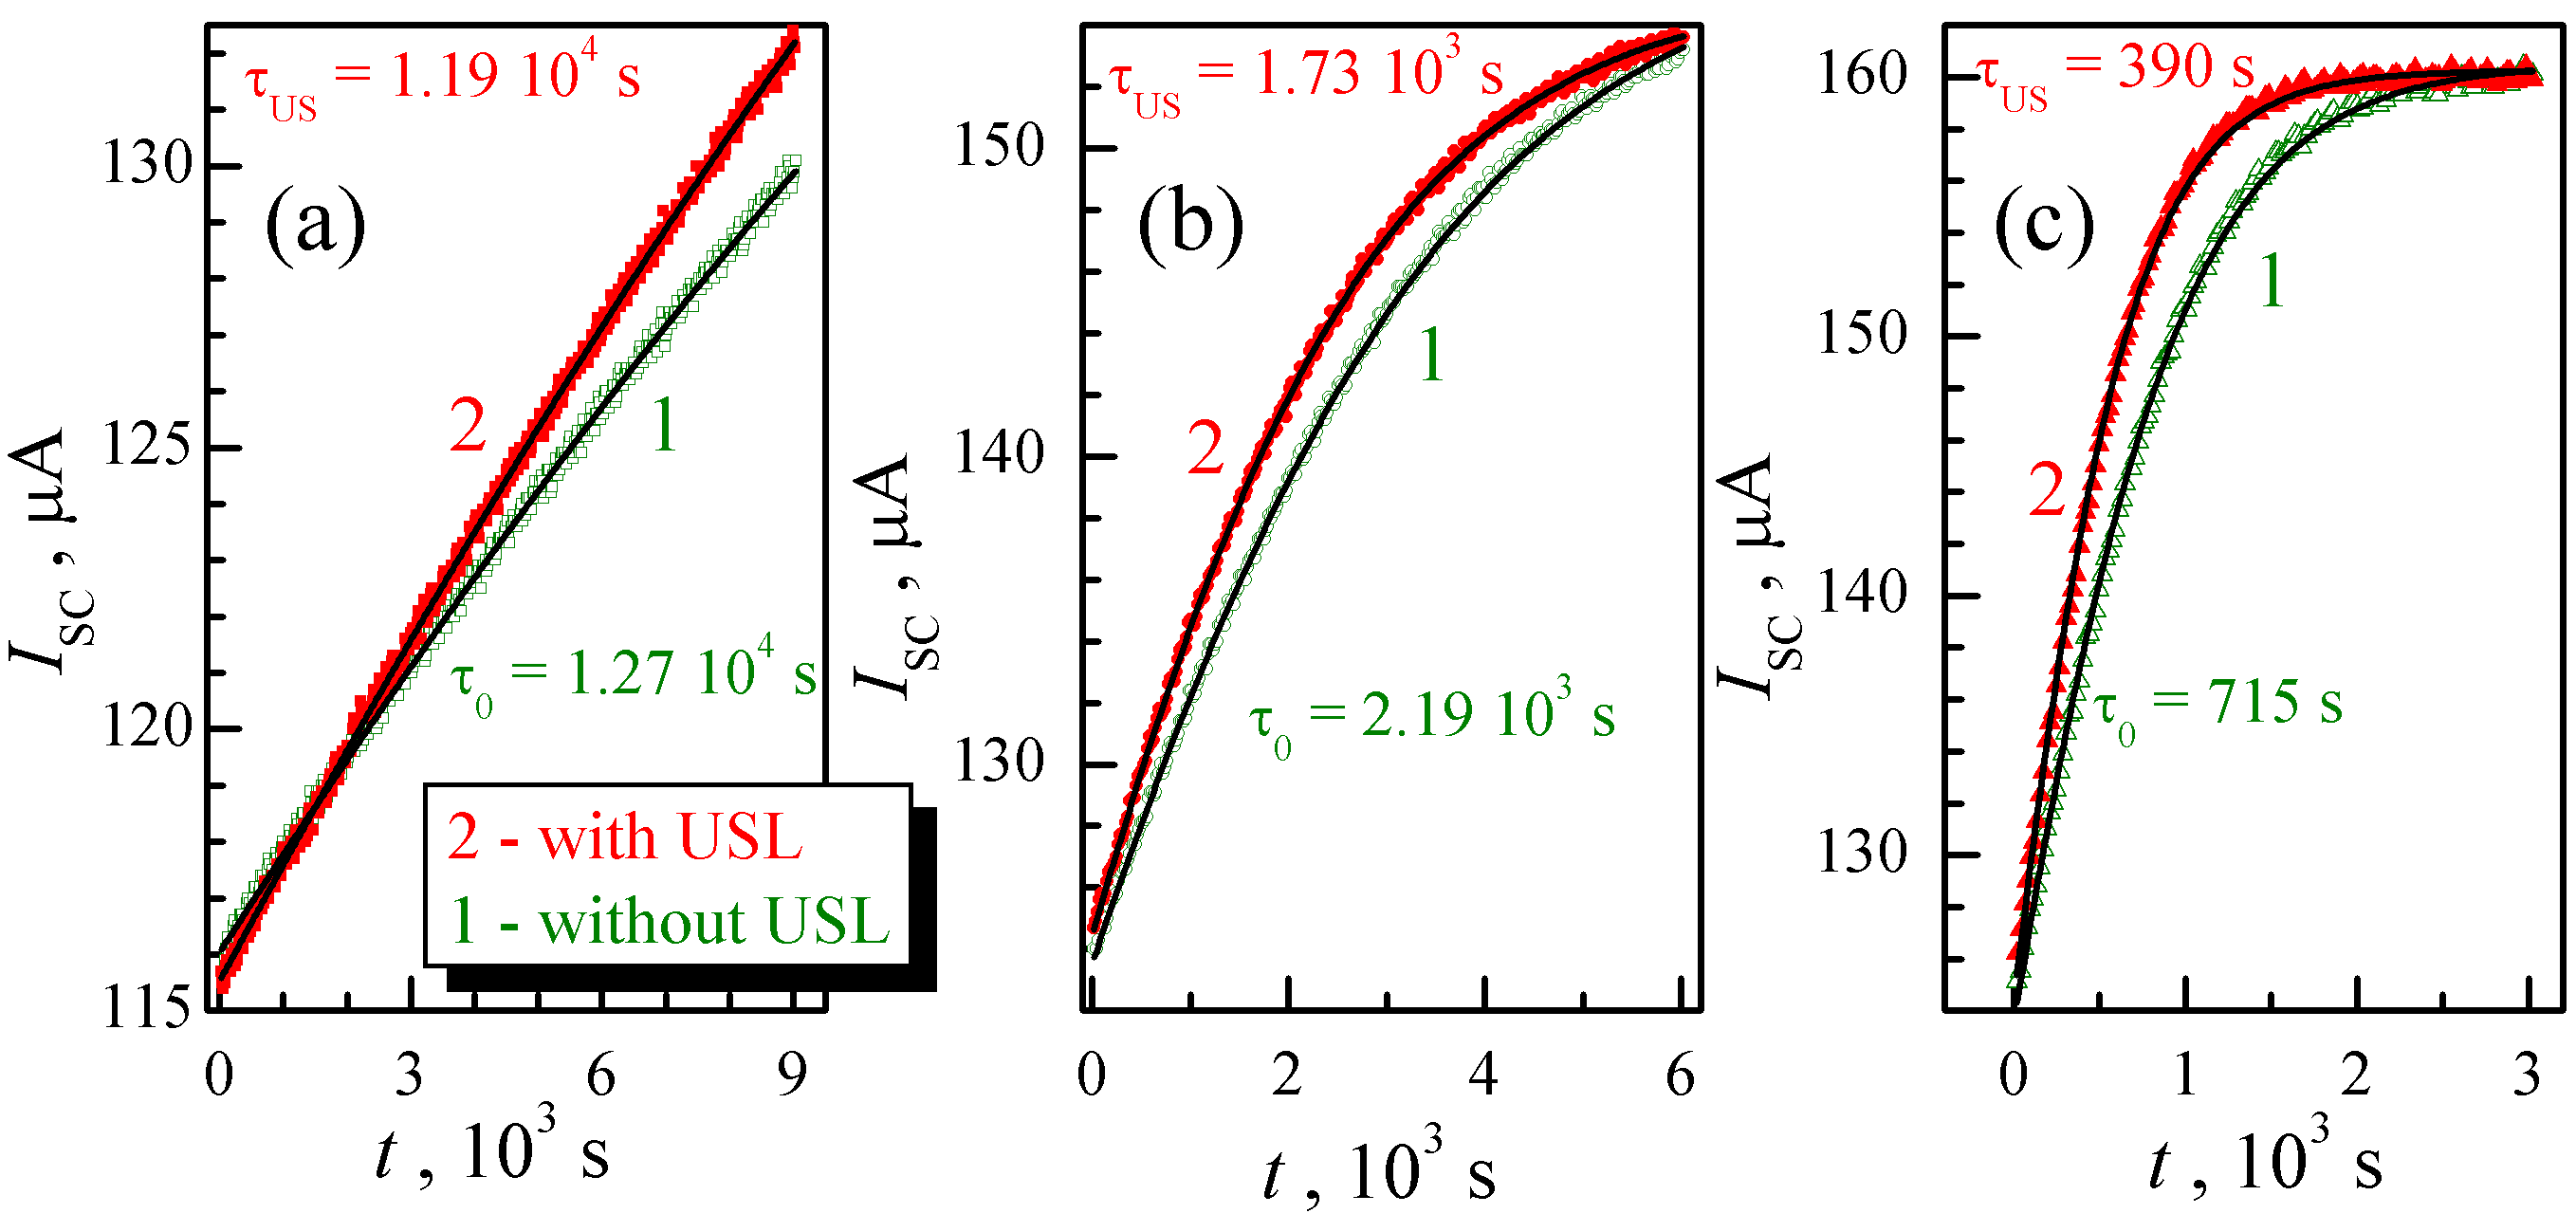
\includegraphics[width=1.0\textwidth]{Fig3}
\caption{
%Kinetics of short circuit current  after intensive illumination under USL
%($f_\mathrm{US} = 2.4$~MHz, filled red marks on the chart)
%and without USL (empty green marks).
%Solid lines indicate fitting according to Eqs.~(\ref{eqIsc})-(\ref{eqNFeBt}).
%$T$, K: 300 (a), 320 (b), 340 (c)
\hl{Measured short circuit current plotted as a function of the time after high-intensive} illumination
under USL (1, filled red marks, $f_\mathrm{US} = 2.4$~MHz) and without USL (2, empty blue marks).
The lines are the fitted curves using Eqs.~(\ref{eqIsc})-(\ref{eqNFeBt}).
$T$, K: 300 (a), 320 (b), 340 (c).
\hl{The pair formation time constants determined by the fitting are shown as well;
$\tau_\mathrm{US}$ (red) --- with USL and $\tau_{0}$ (blue) --- without USL}
}
\label{figIscUs}       % Give a unique label
\end{figure}

The investigations show that the degree at which the association accelerates
under USL depends on acoustic wave intensity.
Fig.~\ref{figfus} gives the data that evidence about decrease
in $\tau_\mathrm{US}$ due to increase in $W_\mathrm{US}$.
It is evident that whatever the US frequency is, $\tau_\mathrm{US}/\tau_{0}$
practically linearly depends on the intensity at small values of $W_\mathrm{US}$.
As USL becomes more intense, the saturation of $\tau_\mathrm{US}$ is observed,
which corresponds to about 0.7$\tau_{0}$.

\begin{figure}
\centering
 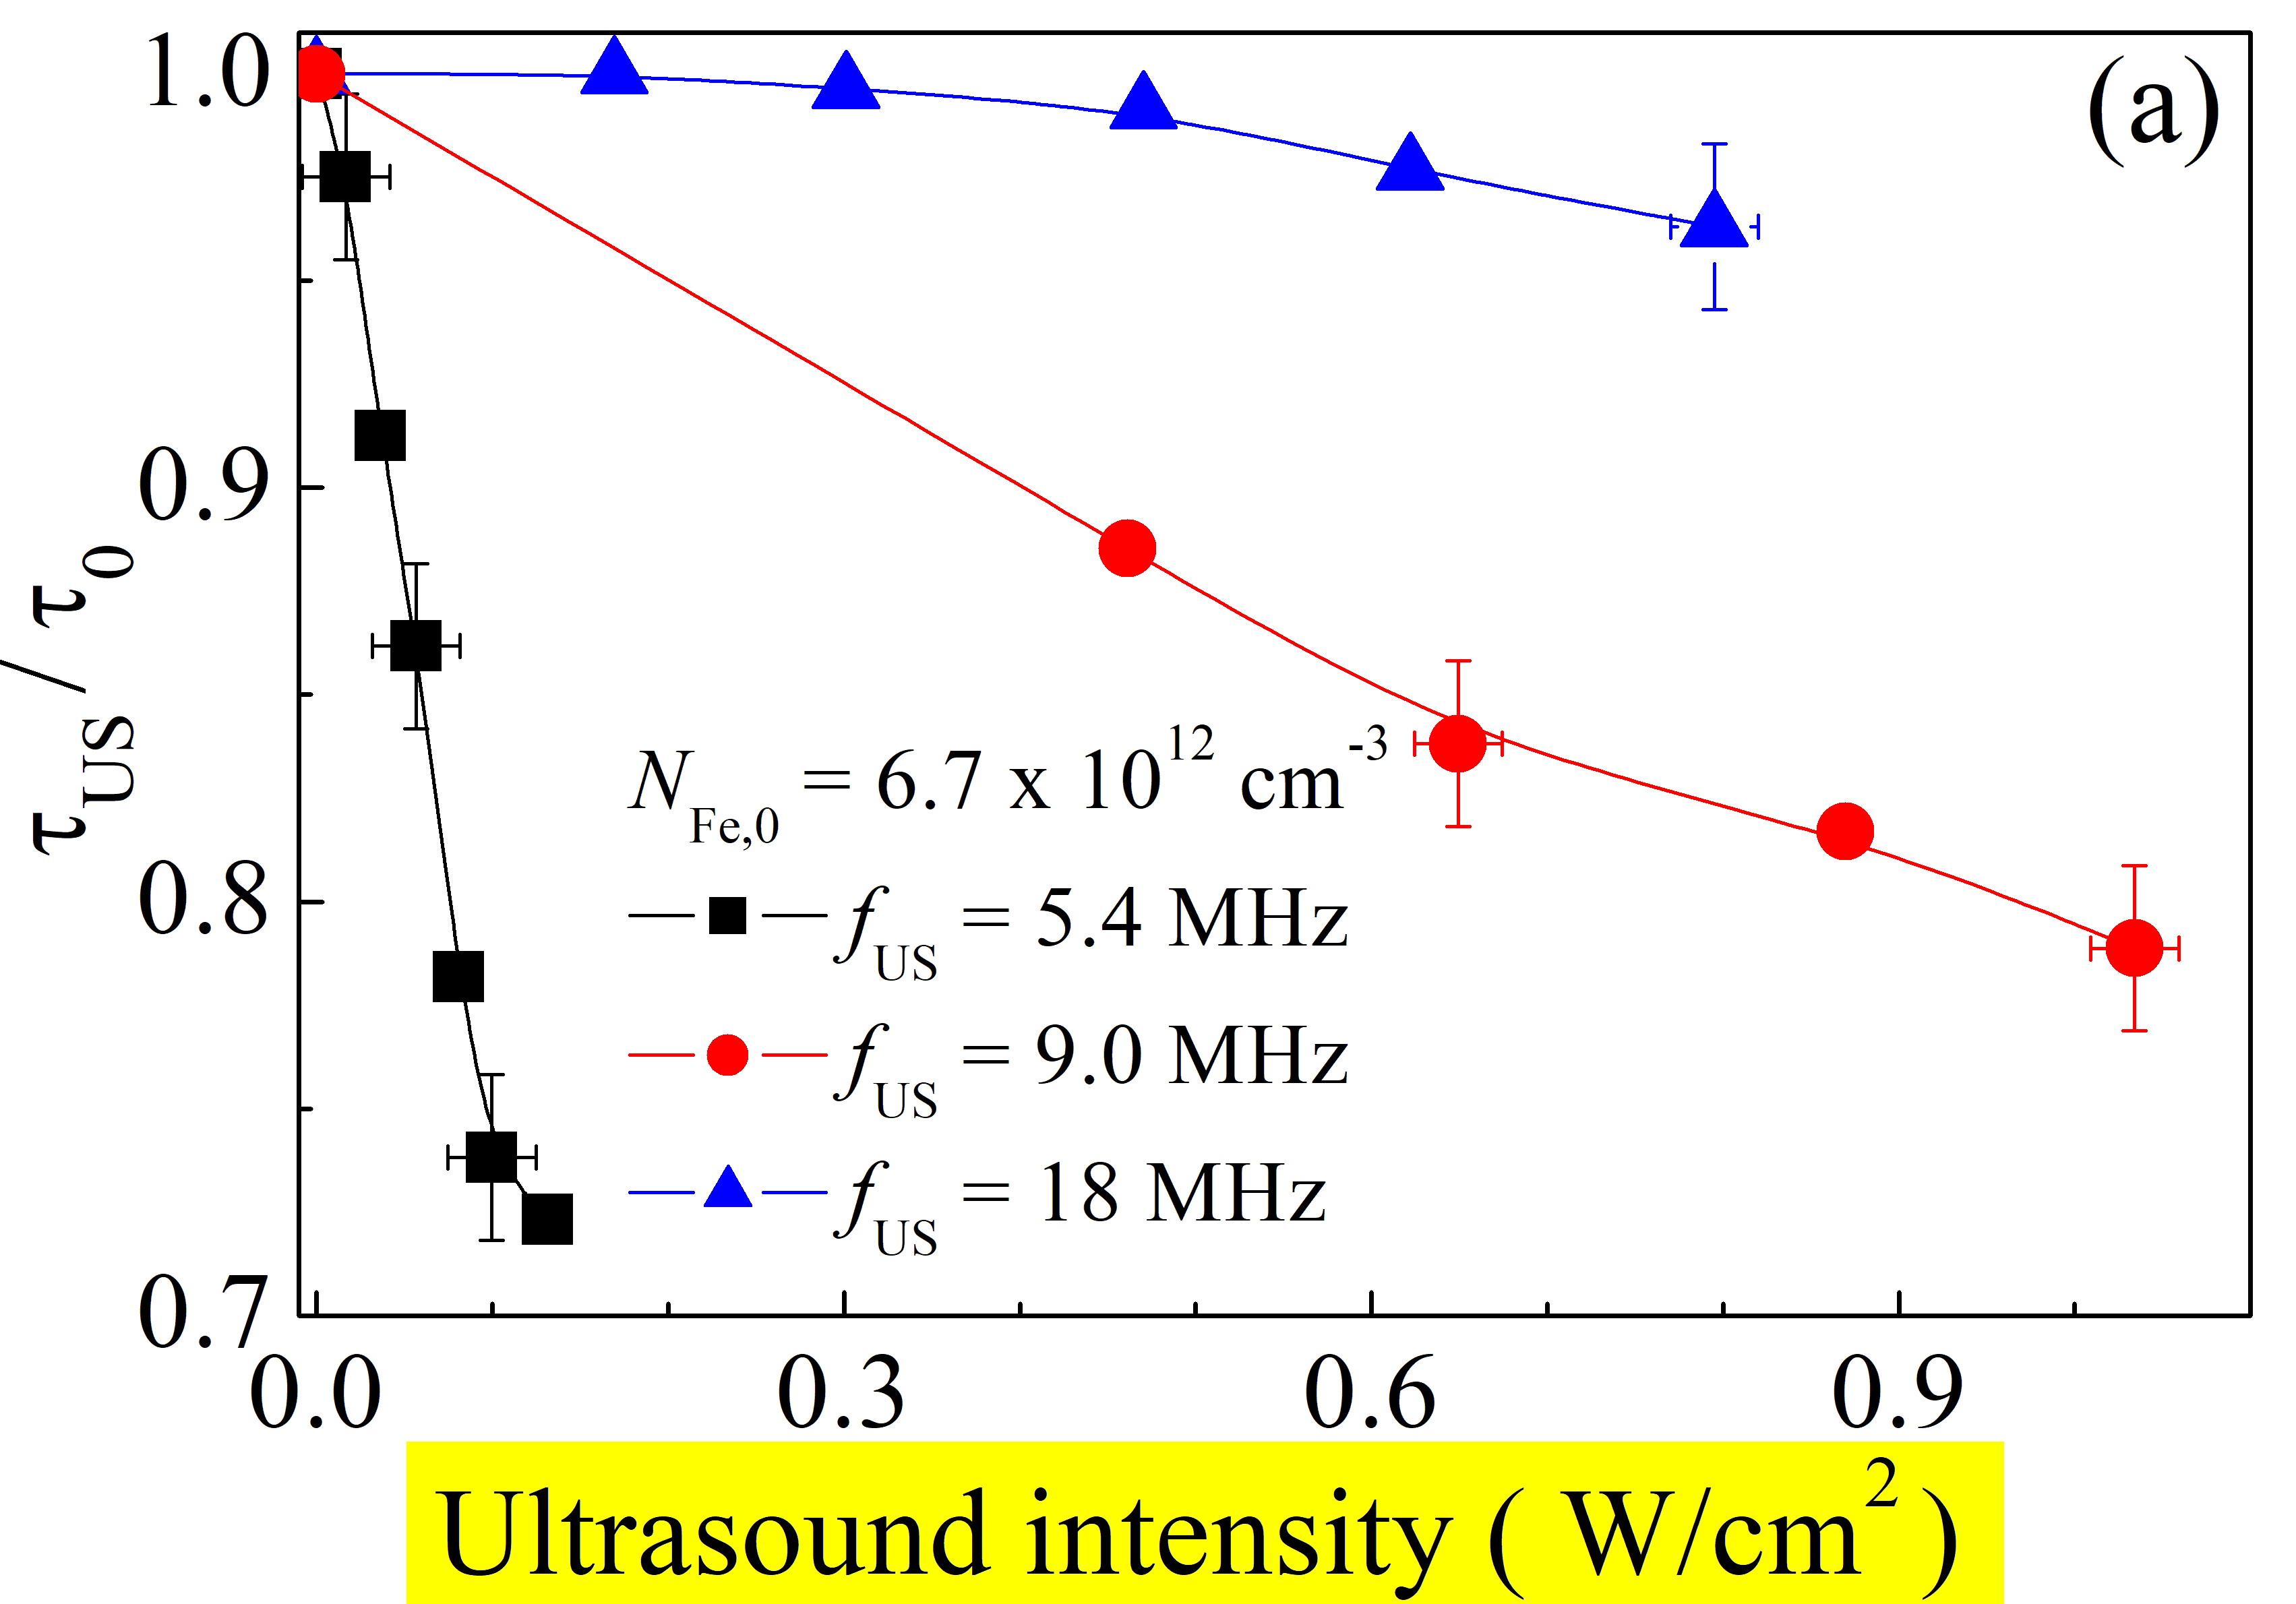
\includegraphics[width=0.45\textwidth]{Fig4a}
 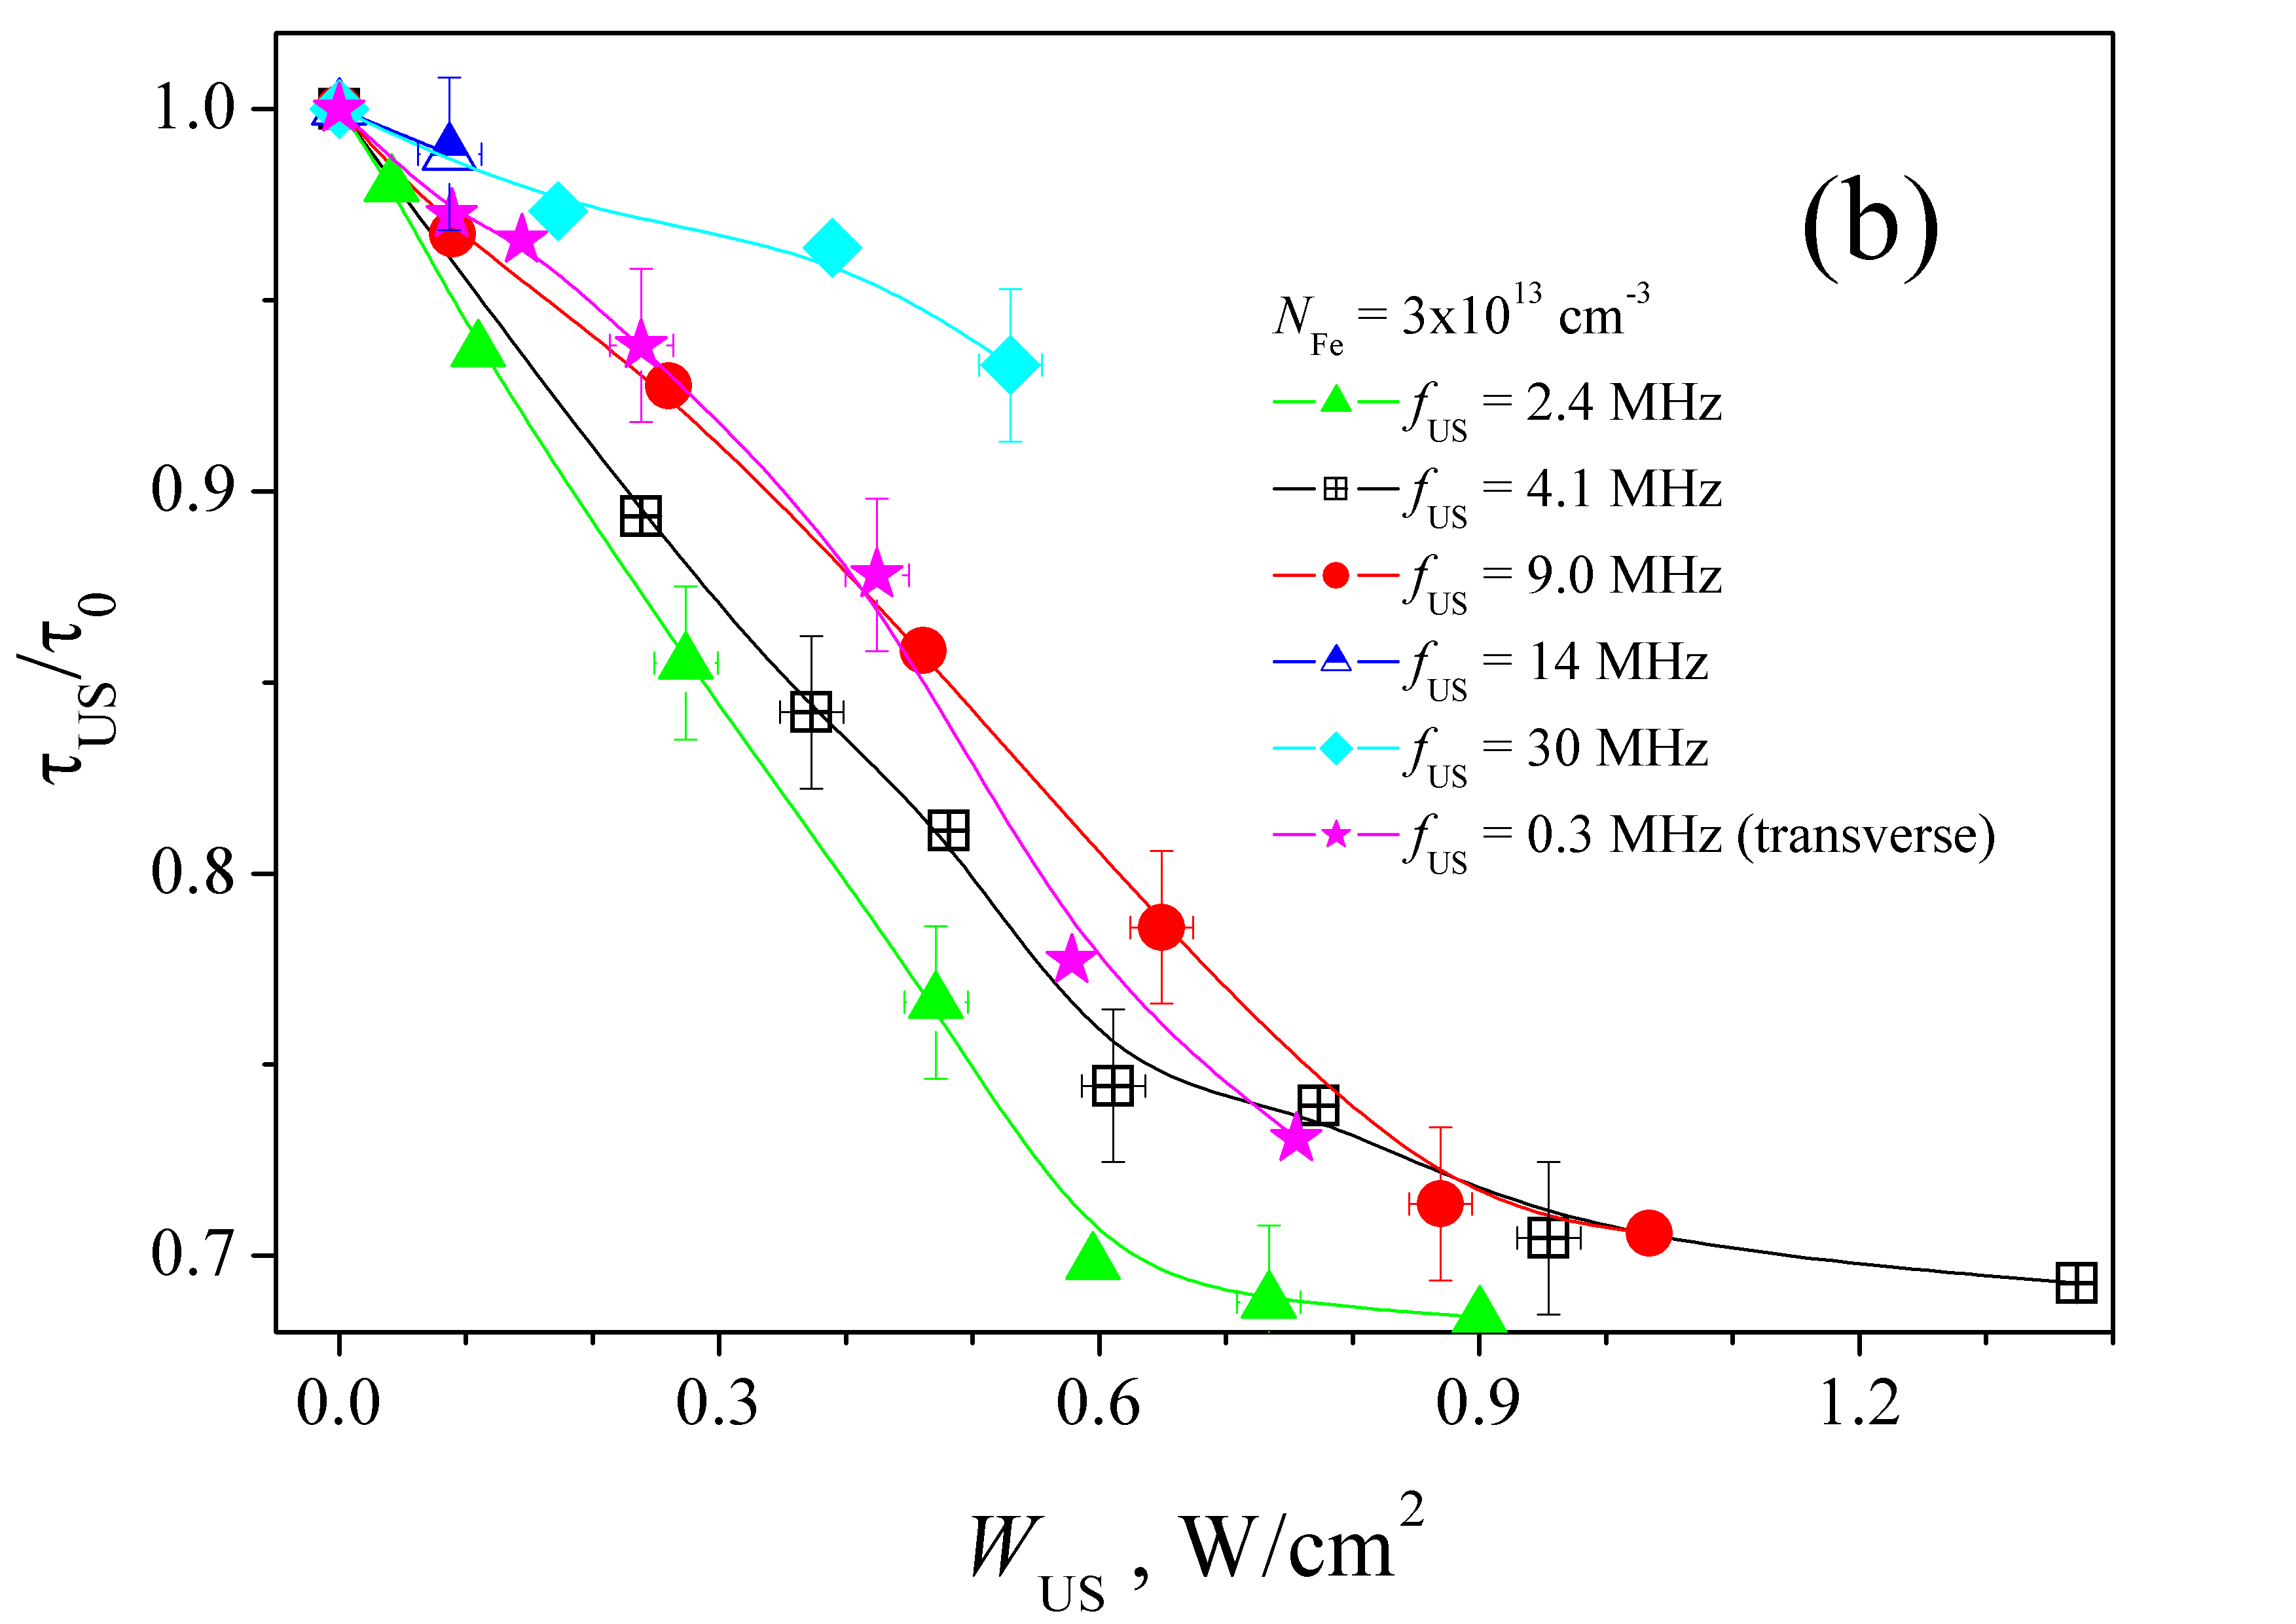
\includegraphics[width=0.45\textwidth]{Fig4b}
\caption{
The dependencies of the degree of AI time decrease on the applied US intensity at different $f_\mathrm{US}$.
Parts a and b present the samples with different iron concentrations.
$T=340$~K.
The marks are the experimental results, the lines are given for convenience only
}
\label{figfus}       % Give a unique label
\end{figure}

Also, Fig.~\ref{figfus} demonstrates that the efficiency of
AI change in migration energy decreases as the US frequency increases,
this effect being observed for all the samples and does not depend on impurity iron concentration.
In particular, saturation $\tau_\mathrm{US}/\tau_{0}$ at $f_\mathrm{US}=2.4$~MHz is observed
at approximately $W_\mathrm{US}=0.6$~W/cm$^2$,
while for $9.0$~MHz it is revealed at $0.9$~W/cm$^2$, see Fig.~\ref{figfus}(b).
As for the saturation magnitude, it does not depend on $f_\mathrm{US}$.
Transverse waves, despite lower frequency, more weakly impact the processes of \hl{FeB pair association.
It is previously shown} \cite{Olikh2018SM} \hl{that the acoustically-induced change of complex defect parameters can be attributed to the variation in the distance of the components, and this effect is intensified in the case of the transverse waves.
The opposite feature of investigated phenomenon testifies that the AI acceleration of the FeB pair
association does not deal with iron-boron distance change.}

Fig.~\ref{figfus} also gives iron concentrations $N_\mathrm{Fe,0}$ obtained from $I_\mathrm{SC}$ relaxation
in conditions of complete pair dissociation (i.e. the illumination that causes the maximum short circuit current decrease).
The next figure, Fig.~\ref{figNFe}, presents $\tau_\mathrm{US}/\tau_{0}$  dependencies
for the samples with different iron concentrations under USL of the same US frequency.
It is evident that the magnitude of AI effect in fact does not depend on $N_\mathrm{Fe,0}$.

\begin{figure}
\centering
 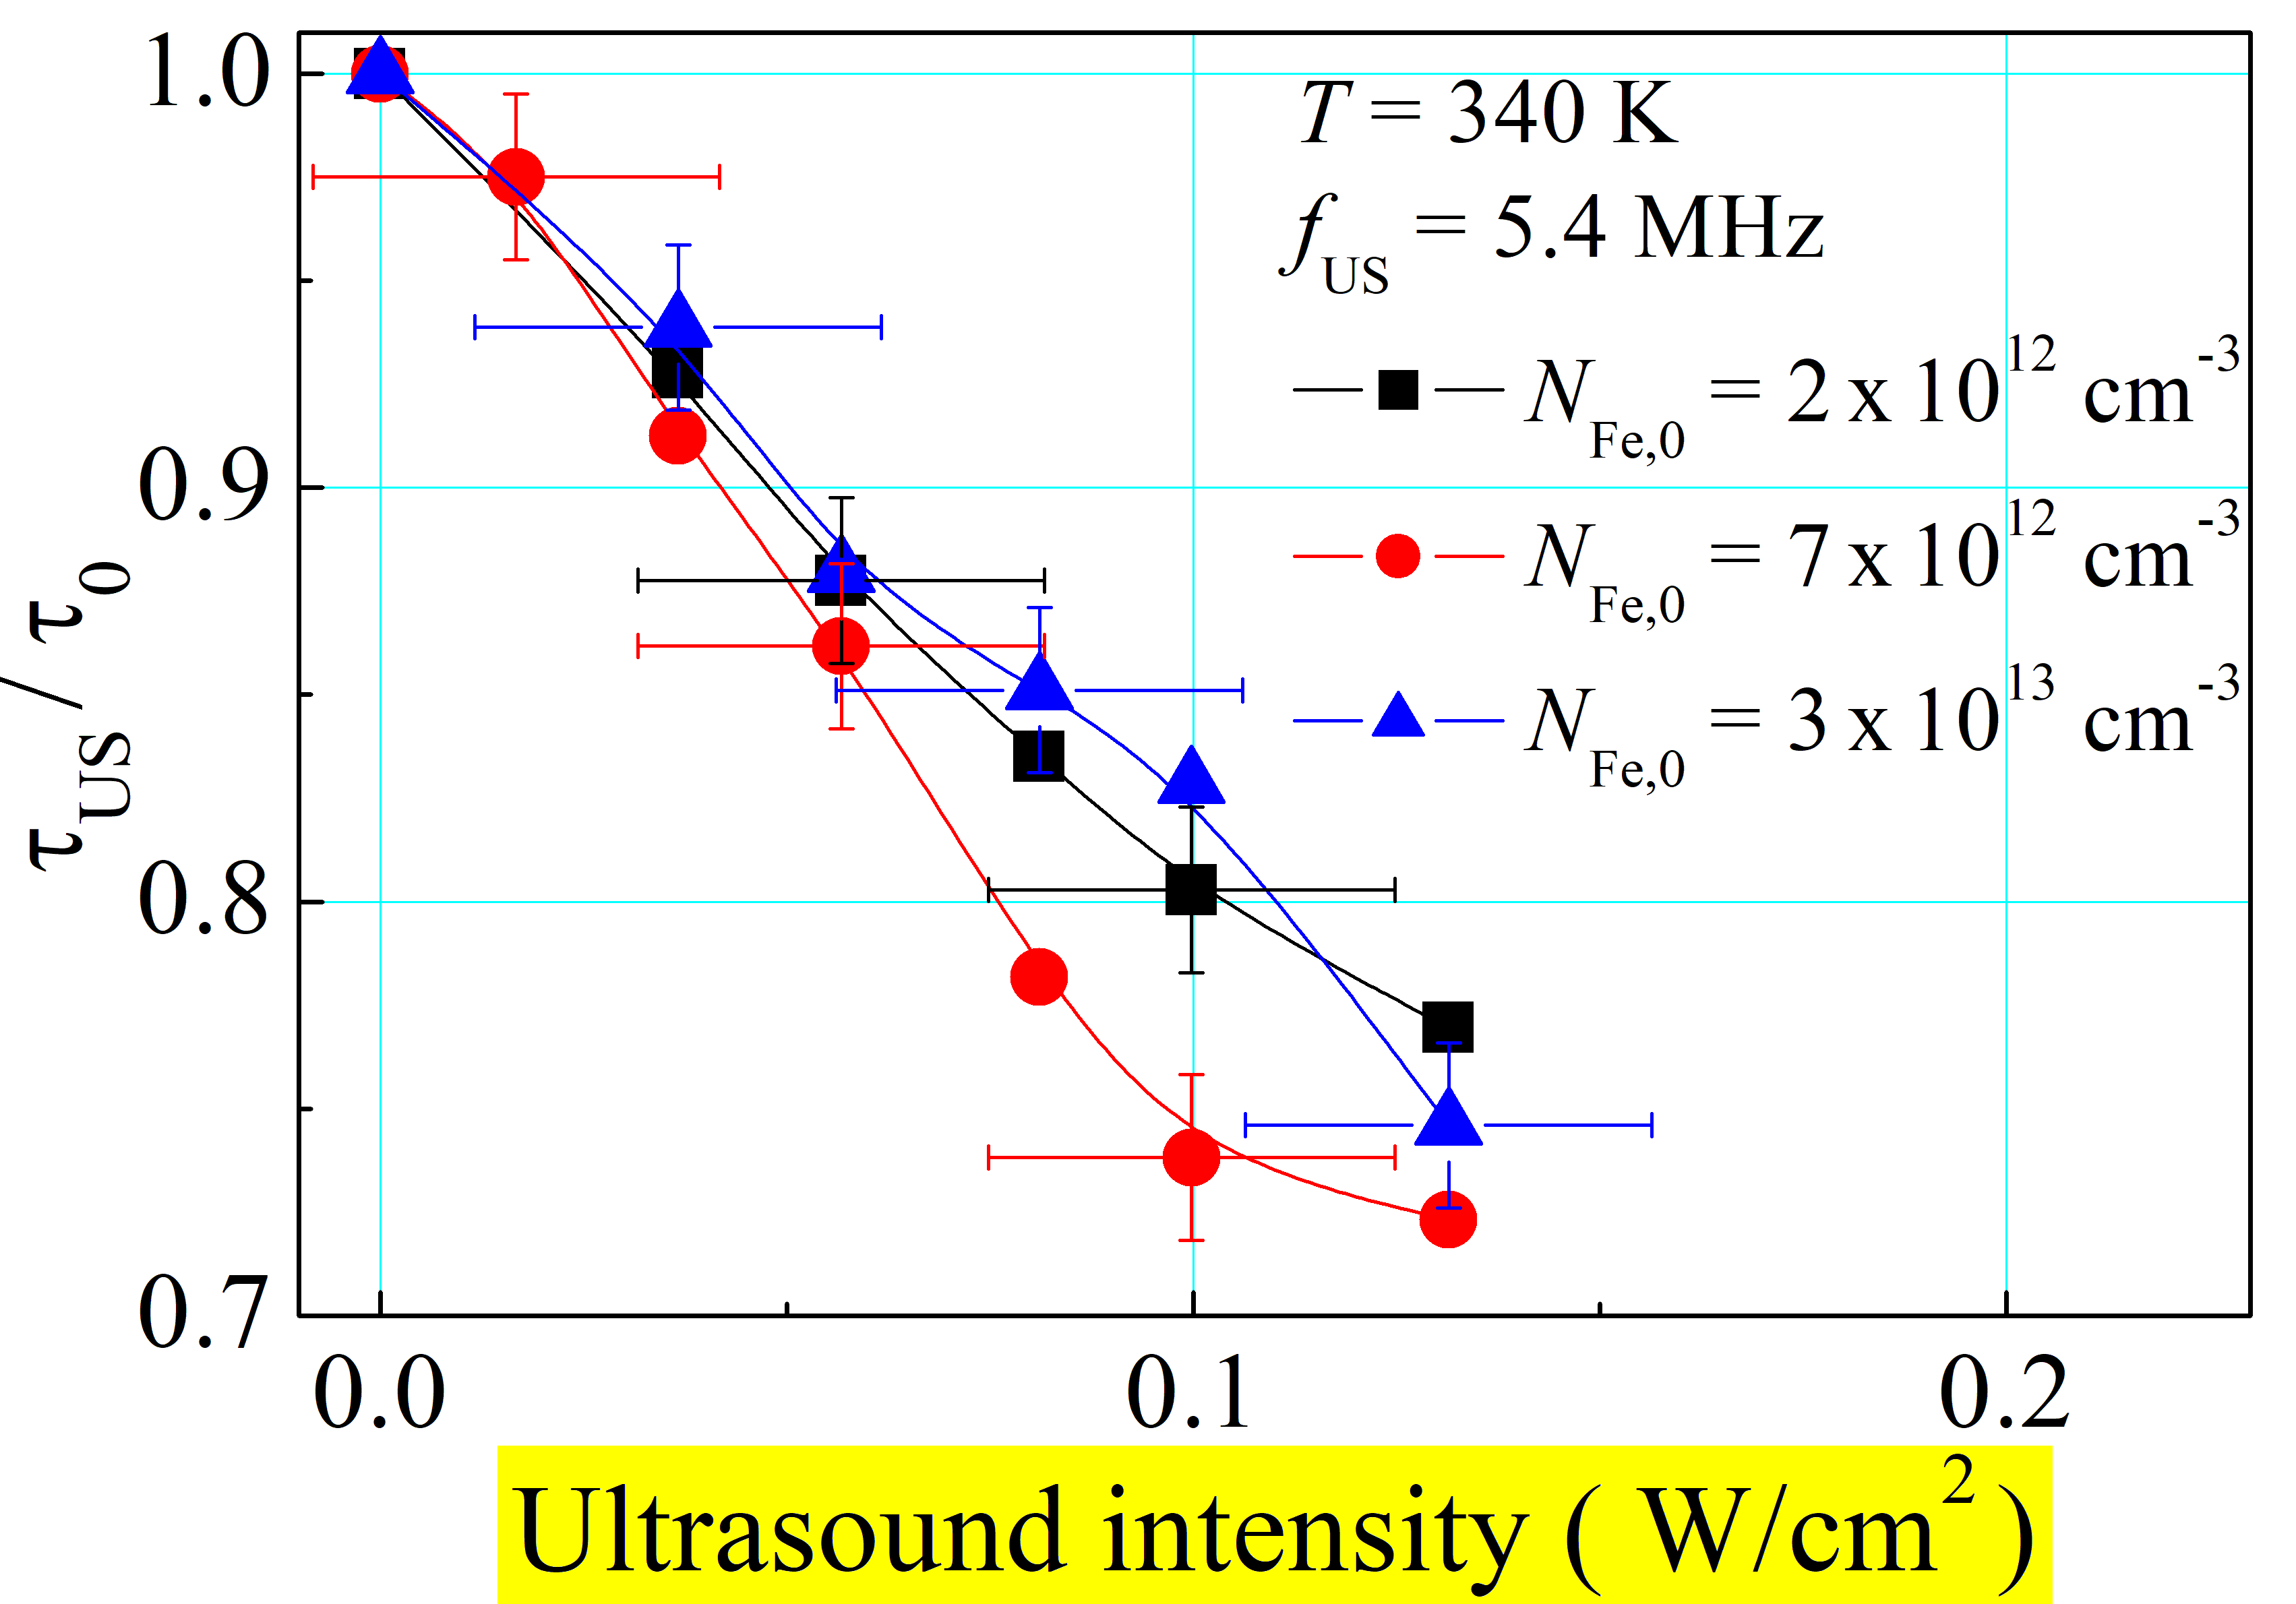
\includegraphics[width=0.5\textwidth]{Fig5}
\caption{
The dependencies of the degree of AI association time decrease on applied US intensity
in SC with different content of iron atoms.
$T=340$~K.
$f_\mathrm{US}=5.4$~MHz.
The marks are the experimental results, the lines are given for convenience only
}
\label{figNFe}       % Give a unique label
\end{figure}

Our experiments have shown that
as the temperature decreases the efficiency of US impact on $\tau_{ass}$ increases
(see Fig.~\ref{figTemp} which presents the temperature dependence of $\tau_\mathrm{US}/\tau_{0}$)
at a constant intensity of US application.
In general, these curves are close to linear.

\begin{figure}
\centering
 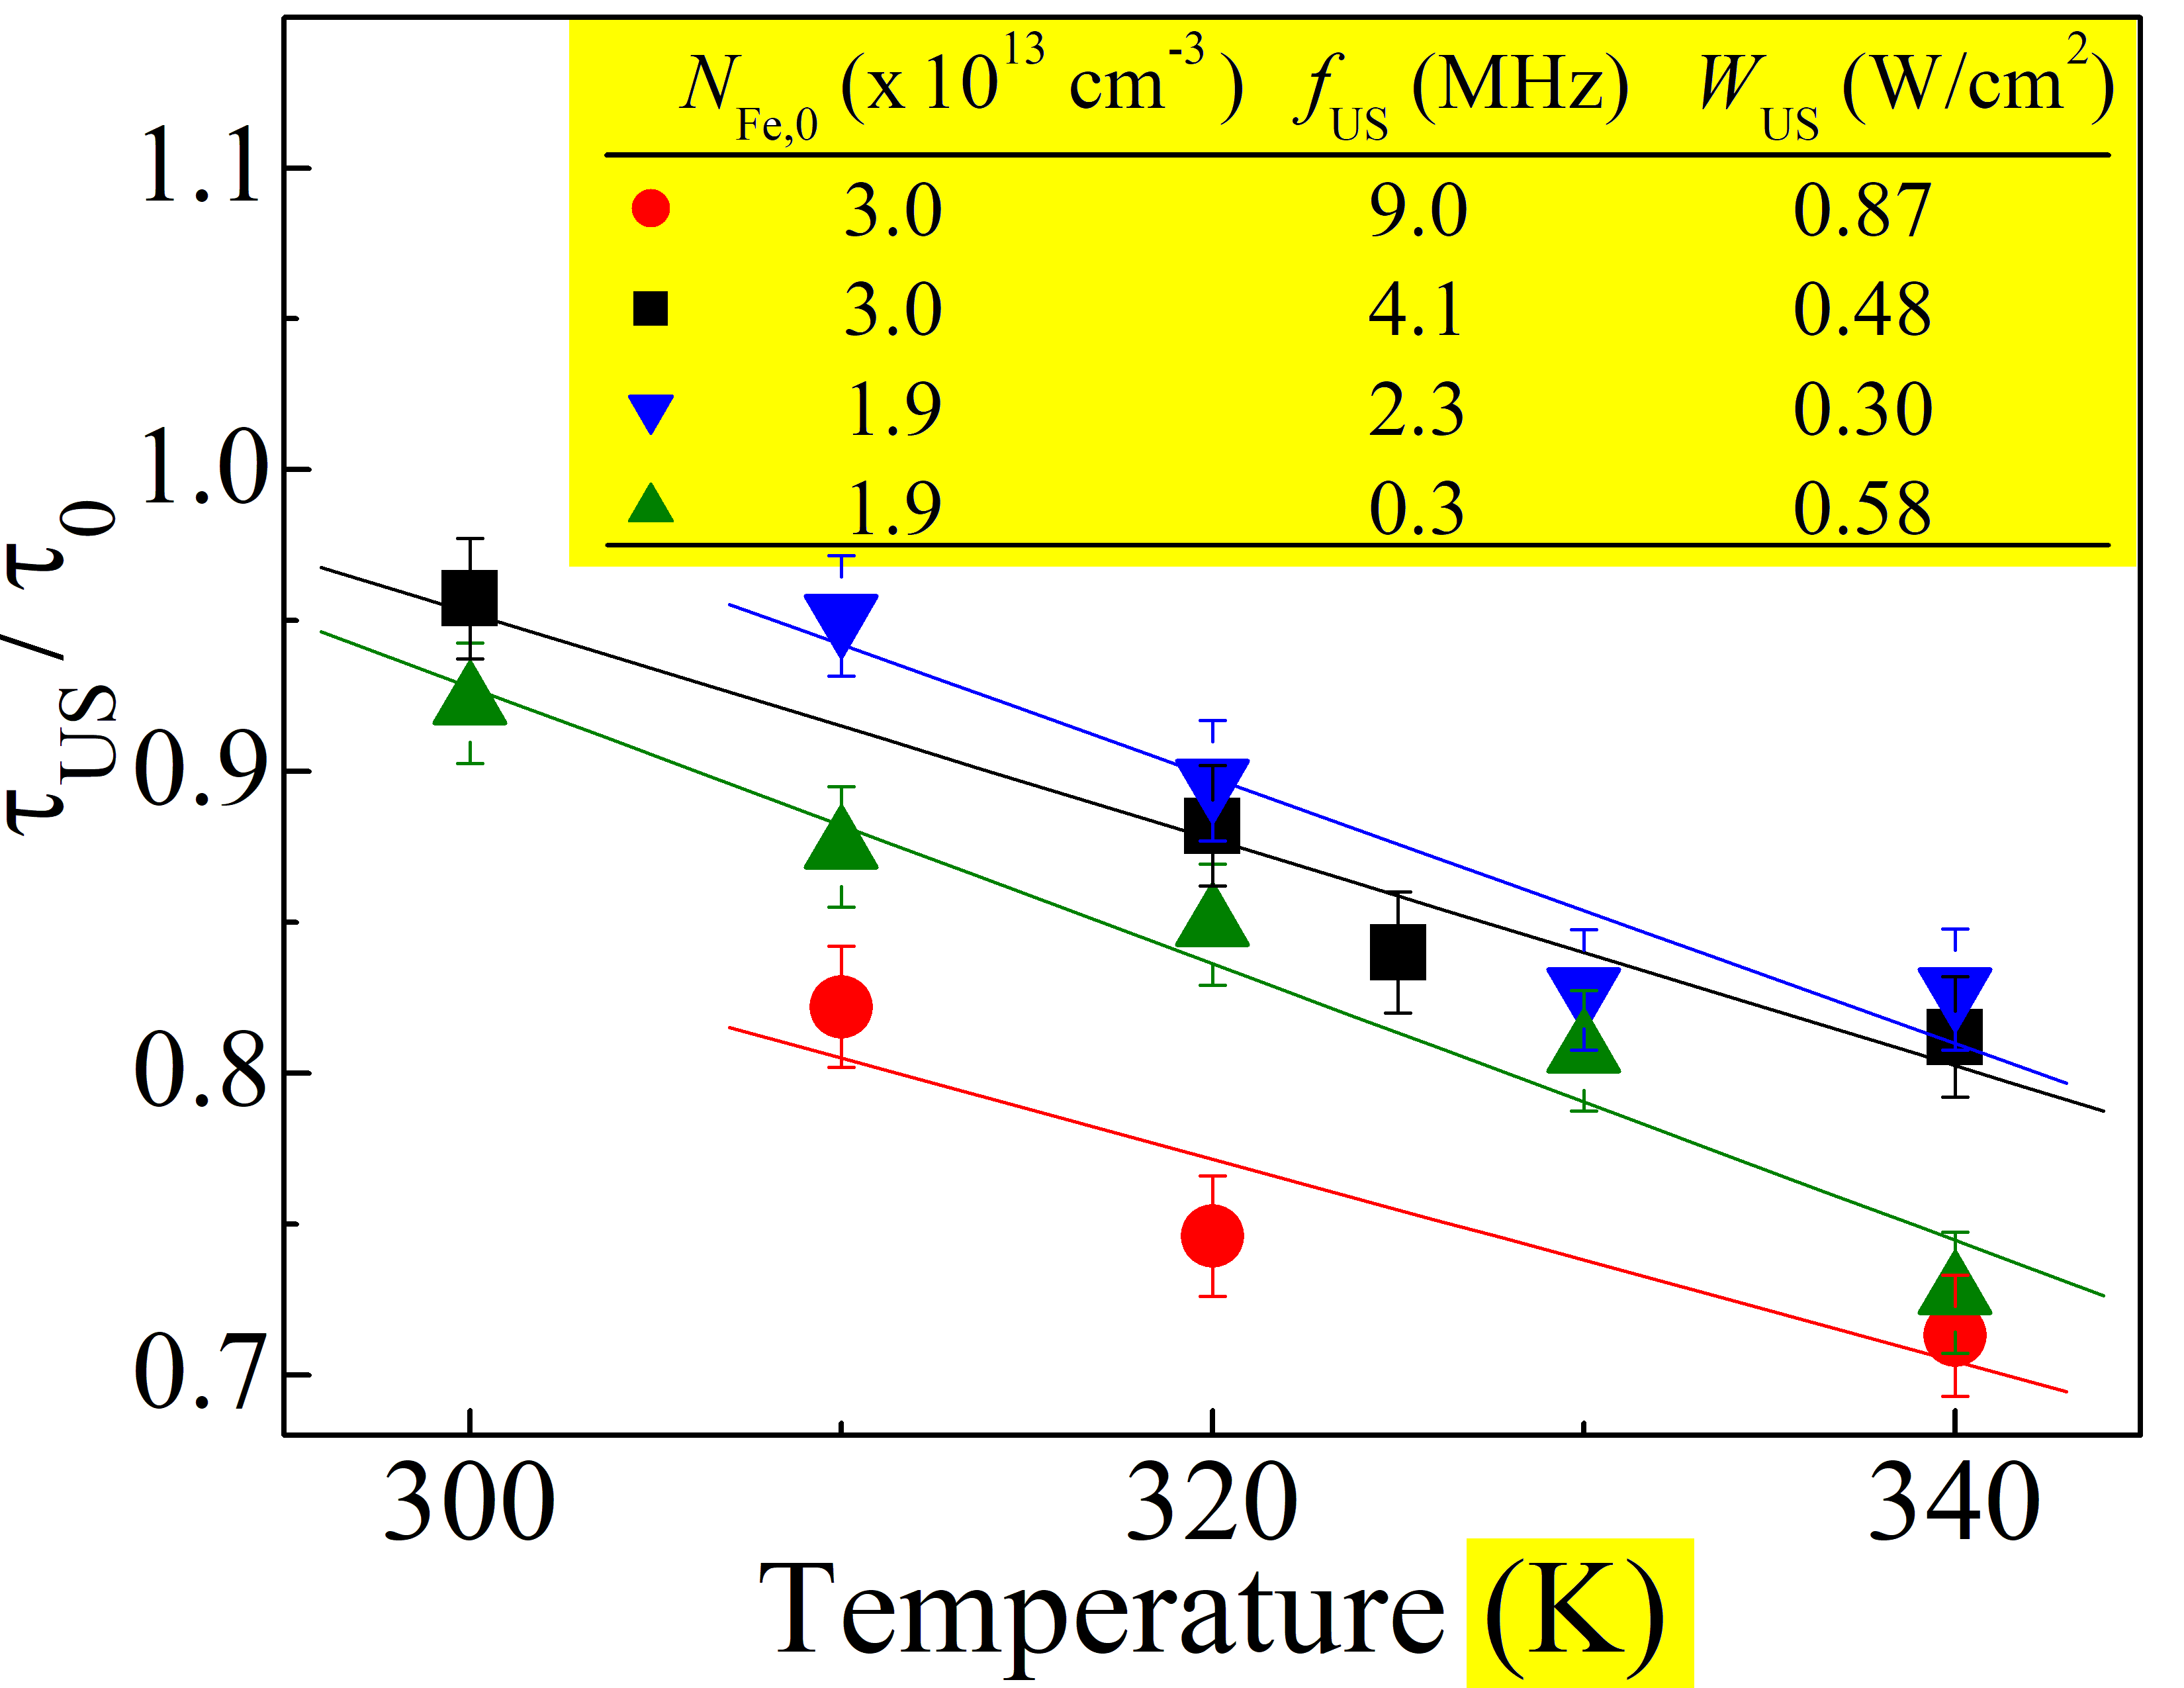
\includegraphics[width=0.5\textwidth]{Fig6}
\caption{
Temperature dependencies of  acoustically induced FeB association time decrease.
The marks are the experimental results, the lines are the linear fitted curves
}
\label{figTemp}       % Give a unique label
\end{figure}

The association of FeB complex happens at the  expense of  Fe$_i$ diffusion towards the
boron atoms located in substituting positions and strongly bound with the neighbour due to forming covalent bonds with them.
Therefore, the $\tau_{ass}$ depends on the coefficient of iron diffusion $D_\mathrm{Fe}$,
so a more detailed, in comparison with Eq.~(\ref{eqTass}), expression takes the following form \cite{FeBAssJAP2014,FeBJAP2005,FeBKin2019}:
\begin{equation}
\label{eqTass2}
\tau_{ass}=\frac{\varepsilon\varepsilon_0 kT}{q^2D_\mathrm{Fe}N_A}=
\frac{\varepsilon\varepsilon_0 kT}{q^2D_\mathrm{0,Fe}N_A}\exp\left(\frac{E_m}{kT}\right)\,,
\end{equation}
where
$D_\mathrm{Fe}=D_\mathrm{0,Fe}\exp(-E_m/kT)$,
$D_\mathrm{0,Fe}$ is a temperature-independent multiplier,
in the general case \cite{AZIZ2001,Stavola,WeberFe}
$D_\mathrm{0,Fe}=\beta\nu a^2\exp(\delta S_\mathrm{Fe}/k)$,
$\beta$ is a correlation factor,
$\nu$  is an effective vibrational (attempt) frequency,
$a$ is a jump distance,
$\delta S_\mathrm{Fe}$ is the migration entropy.

As evident from Eq.~(\ref{eqTass2}), the decrease in FeB association time under USL testifies about
AI increase in $D_\mathrm{Fe}$.
It is, most probable, due to the increase in diffusion energy (see Fig.~\ref{figUSChem}).
Enhanced diffusion of impurities in the US field was observed previously
both in poly- and mono-crystals of silicon and gallium arsenide \cite{Ostapenko1999,Zaveryukhin2002}.
The decrease in interstitial iron atom migration energy can be given as
\begin{figure}
\centering
 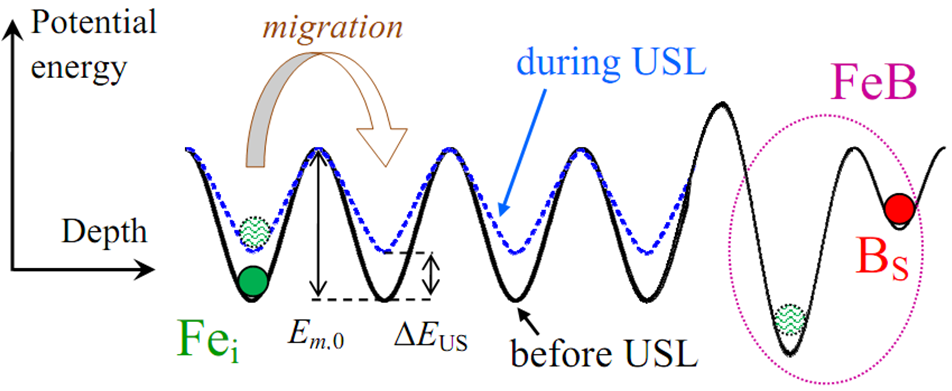
\includegraphics[width=0.9\textwidth]{Fig7}
\caption{
A schematic picture showing the spatial variation of the potential energy of
iron interstitial atom in Si as a function of position near the boron substitutional atom.
US stress lowers the energy barrier for Fe migration.
The curves are scaled arbitrarily
}
\label{figUSChem}       % Give a unique label
\end{figure}

\begin{equation}
\label{eqEmUs}
E_m \xrightarrow{ultrasound} E_{m,0}-\Delta E_\mathrm{US}\,,
\end{equation}
where $E_{m,0}$ is the migration energy without elastic oscillations in silicon SC,
which is $E_{m,0}\sim0.66$~eV according to \cite{FeBAssJAP2014,FeBkinAPL2008} and our experimental data;
$\Delta E_\mathrm{US}$ is the AI change in this quantity value.
According to the performed investigations  $\Delta E_\mathrm{US}=f(W_\mathrm{US},f_\mathrm{US},T)$ and does not exceed 10~meV.

The physics of the found AI effect can be the following.
By using thermodynamic formalism it was shown in \cite{AZIZ2001} that the ability of
impurities in Si to diffuse depends on mechanical stress $\eta$:
\begin{equation}
\label{eqTeor}
\frac{D(\eta)}{D(0)}=\exp\left(\frac{\eta V^*}{kT}\right)=
\exp\left(\frac{\eta [-\Omega+V^r+V^m]}{kT}\right)\,,
\end{equation}
where
$V^*$ is an activation strain tensor,
$\Omega$ is the atomic volume representing  crystal dimension changes
upon the formation of lattice site before the lattice relaxation
around the newly created point defect is permitted,
$V^r$ is a relaxation volume,
$V^m$ is a migration strain tensor, which characterizes stress impact on the defect mobility.
The enhance Fe$_i$ diffusivity in the strain field is discussed in \cite{FeStrain} as well.

In our opinion, this is the mechanism, which explains the found US impact on FeB pairs association in silicon SC.
As seen from Eq.~(\ref{eqTeor}), the diffusion coefficient change caused
by the applied stress is thermally  activated, which explains the observed
temperature dependence of AI changes in $\tau_{ass}$.
In addition, generally $V^*$ contains 81 component  \cite{AZIZ2001},
and therefore change in $D$ depends on the direction of atom elastic displacements.
This accounts for less effective AI impact of transverse waves.
It should be noted, that it is the absorption of oscillation energy that the authors \cite{GORB2020,UST:Medvid}
use to reveal the causes of USL impact on defect system in Si--SiO$_2$ structures,
and in particular AI increase in impurities mobility.

The observation reported here opens up new possibilities in manipulating electronic
properties of silicon barrier devices.
For example, as mentioned above, during phosphor diffusion, the iron impurity gettering occurs as well.
This happens at high temperatures (near 900$^\circ$C),
and for this reason iron is found in unpaired interstitial state.
USL applied during this technological process should increase the degree of the SC basic region
cleaning due to AI increase in Fe coefficient and as a result improve SC performance.

\section{Conclusion}

The ultrasound influence on
FeB pair association in silicon solar cells has been investigated experimentally.
The investigation has revealed that pair associations are accelerated due to enhance of iron
atom diffusion under the action of ultrasound field.
The effect gets stronger with the increase in temperature and decrease in USL frequency.
The application of longitudinal waves is more effective than that of transverse waves.
The effect can be related to a nearly room--temperature decrease in iron migration energy (to 10 meV) in the ultrasound stress fields.
Thus, ultrasound can be an effective functional tool for controlling silicon structure characteristics.


\backmatter


%\bmhead{Acknowledgments}
%
%The authors would like to acknowledge the financial supports by National Research Foundation  of Ukraine
%(project number 2020.02/0036)

\section*{Statements and Declarations}

\bmhead{Conflict of interest}
There are no conflicts to declare.

\bmhead{Data availability statement}
Some or all data generated or used during the study are available from the corresponding author by request.

\bmhead{Funding}
This work was supported by National Research Foundation  of Ukraine (project number 2020.02/0036).

\bmhead{Author Contributions}
All authors contributed equally to this work.

%Some journals require declarations to be submitted in a standardised format. Please check the Instructions for Authors of the journal to which you are submitting to see if you need to complete this section. If yes, your manuscript must contain the following sections under the heading `Declarations':
%
%\begin{itemize}
%\item Funding
%\item Conflict of interest/Competing interests (check journal-specific guidelines for which heading to use)
%\item Ethics approval
%\item Consent to participate
%\item Consent for publication
%\item Availability of data and materials
%\item Code availability
%\item Authors' contributions
%\end{itemize}
%
%\noindent
%If any of the sections are not relevant to your manuscript, please include the heading and write `Not applicable' for that section.



\bibliography{olikh}% common bib file
%% if required, the content of .bbl file can be included here once bbl is generated
%%\input sn-article.bbl

%% Default %%
%%\input sn-sample-bib.tex%

\end{document}
